\documentclass[11pt]{article}

\usepackage{apacite}
\usepackage{amsmath}
\usepackage{amssymb,enumerate}
\usepackage{bibentry}
\usepackage{rotating}
\usepackage{caption}
\usepackage{array,multirow}

\usepackage[authoryear,round,longnamesfirst]{natbib}

\usepackage{enumitem}
\usepackage{setspace}
\linespread{1}
\usepackage{epsf,graphicx,psfrag}
\usepackage{lipsum}
\usepackage{framed}
\usepackage{graphicx}
\usepackage[export]{adjustbox}
\usepackage{geometry}
 \geometry{
 a4paper,
 total={210mm,297mm},
 left=25mm,
 right=25mm,
 top=25mm,
 bottom=25mm,
 }
\usepackage{pdflscape}
\usepackage{array}% http://ctan.org/pkg/array
\usepackage{color, colortbl}
\definecolor{Gray}{gray}{0.95}
\definecolor{LightGray}{gray}{0.85}
\definecolor{VLightGray}{gray}{0.75}
\definecolor{darkblue}{rgb}{0.0,0.0,.7}
\definecolor{shadecolor}{gray}{0.85}
\usepackage{color}
\usepackage{hyperref}
\hypersetup{colorlinks,breaklinks,linkcolor=darkblue,urlcolor=darkblue,anchorcolor=darkblue,citecolor=darkblue}
\usepackage{wrapfig}
\usepackage{CJKutf8}
\newcommand{\zh}[1]{\begin{CJK*}{UTF8}{gbsn}#1\end{CJK*}}

\usepackage{epigraph}
\setlength\epigraphwidth{16cm}
\setlength\epigraphrule{0pt}

\usepackage{etoolbox}
\usepackage{adjustbox}
\usepackage{xr}

\makeatletter
\patchcmd{\epigraph}{\@epitext{#1}}{\itshape\@epitext{#1}}{}{}
\makeatother

\interfootnotelinepenalty=10000
\usepackage{footnote}

\usepackage{float}

\title{The Logic of Informational Repression in China\thanks{\normalsize I would like to thank the National Science Foundation (Award \#1747397) and the Rackham Graduate School at the University of Michigan for their generous funding. I would also like to thank my research assistants, Qiwei Lin and Xinyue Xu for their help with text annotation and edits to survey questions. I would also like to thank Luciana Cingolani, Sasha de Vogel, Iza (Yue) Ding, Yilang Feng, King-Wa Fu, Yuequan Guo, Guo'er Liu, Ting Luo, Steven Moore, Jeffrey Javed, Aofei Lu, Walter Mebane, Jennifer Pan, Daniela Stockmann, Daniel Slater, Michael Thompson-Brusstar, Nicholas Valentino, and Nicole Wu for their helpful feedback.}\\ \large }

\author{Blake\ Miller\thanks{\normalsize{Assistant Professor, London School of Economics} (Email: \mbox{b.a.miller@lse.ac.uk})}}

\date{\today}

\newcommand{\cmmnt}[1]{}

\begin{document}
\maketitle

\begin{abstract}
\begin{normalsize}
In China, the state has fundamentally changed its information control strategies in response to the growing threat of virality on social media. In this paper, I outline the strategy of informational repression that has been developed to combat this threat through cooperation between the state and internet communication technology companies (ICTs). Informational repression is a combination of covert information control and targeted repression. Dominant ICTs in China have increased linkages with state institutions, allowing surveillance and repression of carefully selected targets, and strategic cooptation of individuals with considerable influence on social media platforms. These dual strategies preserve the responsive and informational affordances of social media while mitigating the threat of social media as a conduit for instability. In this paper, I outline this strategy using evidence from government documents. I then examine how this strategy works using series of online experiments conducted in China. I find that keeping information control covert is in both the government and private companies’ best interests. These findings suggest that careful and covert information control, when paired with targeted repression, can mitigate the threat of virality while also limiting backlash and chilling effects that can result from heavy-handed censorship.
\end{normalsize}
\end{abstract}
\doublespacing

\section*{Introduction}

In China, the state has been experimenting with public opinion guidance in online social platforms for over two decades \citep{wei2015gongan,zou2015wangluo,xie2011zhongguo,xie2018zhongguo}. Over this period, the state has employed a mixed-strategy approach to information control, fitting into three main categories: content removal, content augmentation, and targeted repression. In this paper, I argue that the state and internet communication technology companies (ICTs) have converged upon a strategy of “informational repression” that targets individuals covertly, leaving as light a footprint as possible. This is a significant departure from the widespread untargeted repression and censorship of the Mao- and early-Reform periods, and the categorical repression of the post-Tiananmen period. Through a period of contestation with social media companies, the state gained an appreciation of softer, more targeted forms of repression and censorship. Because this approach increases impressions of pluralism and discourse competition in citizens’ online interactions, the state has benefitted from opinion mining of citizens who are less hesitant to speak frankly online. At the same time, the state has learned to leverage the technological expertise of social media companies whose business model relies on effective surveillance of users’ consumer preferences. Fine-grained surveillance of online behavior by technology companies is also useful for determining where the state should direct its repressive efforts. Leveraging digital surveillance for careful targeting of individual targets of repression benefits the state in two key ways. First, it limits the visibility of state interventions, giving individuals a perception of pluralism and discourse competition, and increasing their willingness to share their true opinions. Second, by carefully selecting citizens as targets of repression and censorship, the state avoids widespread backlash and chilling effects that often follow more brute-force, heavy-handed, or categorical censorship and repression.

In this paper, I focus on the first of these two benefits: how individuals respond to covert forms of repression in ways that benefit the state and ICTs alike. First, I trace the evolution of state-involvement in—and contestation between the state and ICTs in China. I argue that through this contestation, a state strategy of informational repression has emerged. The strategy of informational repression combines digital surveillance for target selection and a preference for more covert forms of repression, which limit the visibility of state intervention, limiting backlash against the state and ICTs, while preserving the appearance of discourse competition online.
\citep{han2015manufacturing,han2015defending,king2016chinese,miller2015automated}

Astroturfers make use of mass stores of social data to influence the behavior and opinion of netizens \citep{zeng2015wangluo, zhou2011weibo}. These data are gathered with software platforms that offer ``public opinion emergency early warning systems,'' and natural language processing technologies that track and quantify discourse about ``hot topics'' \citep[201-228]{zhou2011weibo}. The government also uses information control tactics such as censorship, surveillance, and repression to control what information people can and cannot see.

The way these information control tactics are deployed and their effects on individual behavior and opinion are enormously important for understanding their effect on the 1.4 billion Chinese citizens who experience them. Understanding them, however, is also key to understanding the information politics in countries outside of China both present and future. Though much of opinion guidance technology is being developed for the purposes of Chinese domestic security, it is being exported all over the world. As many as 18 countries are using Chinese-built mass surveillance systems. 36 are using Chinese ``public opinion guidance'' techniques \citep{mozur2019made}. These countries include both democracies such as Germany and autocracies such as Venezuela. Russia\footnote{See \cite{morgus2019analysis}} and Iran\footnote{See \cite{farda2019iran}} have been inspired by Chinese principles of surveillance and information control as they develop domestic information control technologies. The Chinese state has is now more openly expressing an interest in promoting its ideas about internet governance globally \citep{deibert2008geopolitics}, and its efforts to infiltrate and guide opinion globally have garnered the attention of many scholars and policy analysts \citep{diamond2019china,brady2018new}. That being said, this analysis is restricted to the Chinese context. 

Despite the massive scale of China's opinion guidance efforts, very little is known about {\it if} they are effective and {\it how} they might be effective. While a handful of recent works examine how experiencing information control can affect behavior and opinion, they disagree about the state logic of information control and the particular ways in which information control tactics can be effective \citep{han2018contesting,roberts2018censored}.\footnote{\citep{han2018contesting} identifies how the pluralism of Chinese voices online and doubts about the motives of regime critics allows the state to benefit from discourse competition, solidifying their control over online communities through subtle interventions. I explore the behavioral microfoundations underpinning this high-level analysis of state strategy and discourse competition. \cite{roberts2018censored} explored how personally experiencing censorship influenced user behavior and expressed opinions. This study, by contrast, explores the effects of observing the resulting distribution of opinions after an information control tactic has been used.} Some claim that information control is effective because it targets and demobilizes collective action \citep{king2013censorship,king2014reverse,havel1978power,arendt1973origins}. Others claim that information control is effective because it manipulates and demobilizes expression \citep{kuran1991now,wedeen1999ambiguities}. Others claim that information control is effective because it can change opinion through sustained propaganda campaigns \citep{geddes1989sources}. In this study, I examine these many theories of how information control might be effective across the three main types of information control: additive, subtractive, and suppressive, which are all explained in detail in \hyperref[types_info_ctrl]{Section \ref*{types_info_ctrl}}.

For each of these types of information control, I explore a common subtype of information control called covert information control. Covert information control refers to information control tactics that obfuscate the state's identity as the information manipulator. Overt information control, by contrast, refers to information control tactics where the state's role as the information manipulator is visible. Even as this type of information control is becoming more and more common in China, it has not yet been examined systematically. I address this gap in the literature using  survey experiments and a custom-built, realistic, interactive news website with a fully functional comment interface.

% FINDINGS PARAGRAPH

This work gives us a better idea of {\it if} and {\it how} information control tactics can be effective. It is also the first study to measure the causal effect of {\it covert} information control on the magnitude of various measures of ``effectiveness.'' Understanding how commonly-used information control tactics can affect behavior and opinion is important to understanding  politics in the era of surveillance capitalism.As big data that capture measures of individual behavior have become widely available, political actors in democracies and autocracies alike have increasingly made use of these tactics to mobilize and influence public opinion.

\section{Background}

\subsection{Reducing Backlash through Covert Interventions}

{\setstretch{1}
\epigraph{``Any dissemination of information involves an information selection process. During the process, there are a variety of `gatekeepers' such as content editors and webmasters who play a very important role in information selection and opinion guidance. These `gatekeepers' should not simply delete comments but focus on the art of guidance so as to persuade and move the masses.''\footnotemark\newline}{--- {\it Weibo Government Platforms and Responsiveness to Public Opinion} \citep[155]{zhang2014weibowenzheng}}}
\footnotetext{Original Chinese text: ``\zh{任何信息的传播都是信息选择的过程,期间充满了各种各样的“把关人”。网络“把关人”包括网站编辑,网管等,他们在信息选择,引导舆论方面至关重要。这些网络“把关人”在工作中,切记简单粗暴地删帖,注重运用动之以情,晓之以理的引导艺术,使网民产生理性和感情上的认同和共鸣。}''}

The Chinese public has grown accustomed to contestation and pluralism in the public sphere \citep{han2018contesting,lei2019contentious}. While Chinese citizens understand that the state regulates information through censorship and media controls, these restrictions are often not as noticeable or disruptive as one might think. Through years of experimentation with more open and social modes of publication and digital mass-communication, the state has developed a principle of ``guidance'' instead of ``deletion.'' Guidance is a process of subtle interventions to ``channel'' or ``guide'' public opinion without alerting netizens to the state’s interventions.

This principle became widely used and recommended in government manuals after repeated failed interventions, the first being the bungled cover-up of the SARS epidemic. In the manual, {\it Online Public Opinion in Major Emergency Events}, the principle of ``guide, don’t delete'' traces its roots to this crisis. According to this manual, the SARS epidemic demonstrated to the government that lack of information transparency will only escalate an incident’s severity. In the SARS crisis, lack of information transparency and heavy censorship led netizens to doubt the representativeness of the opinions they encountered, ``damaged the image'' of the government and official media, and ultimately led to the spread of conspiracy theories about the epidemic \citep[1-36]{gong2012zhongda}. One government opinion management manual suggests that repeated failed interventions such as the response to SARS ``may ultimately lead to a people’s revolution.'' \citep[259-273]{ren2013yulun}.

To avoid backlash such as that experienced during the SARS crisis, cadres are directed to maintain a semblance of discourse competition in online media: the manual emphasizes that, ``negative information management [should] go past filtering and censorship, and also ensure the free flow of information by encouraging more voices on the internet.'' Interventions should ``guide the public to empathize with the government,'' and empower netizens to take over control of online public opinion \citep[12-15]{zou2015wangluo}. The government has stressed the importance of intervening early in a crisis to set the agenda---usually through co-optation and repression of opinion leaders \citep[180-194][]{zeng2015wangluo,zhou2011weibo}. This ensures that interventions appear more credible to the public as they come from ``disinterested'' peers who appear to be outside of the party and government's direct influence.

Despite the potential threat that new modes of communication pose, autocrats increasingly use the internet and information communication technology to strengthen and legitimize their rule through legislation, information control, and cooptation of private companies \citep{lessig1999code}. New digital mass-surveillance systems have allowed them to target information control more precisely than was previously possible \citep{shahbaz2018freedom}.

\subsection{Types of Information Control}\label{types_info_ctrl}

Information control is the systematic government manipulation of the visibility of information to the public. I suggest three main sub-types of information control based on how one can change the visibility of information: adding favorable information (using astroturfing, propaganda, etc.), subtracting unfavorable information (through deletion, shadow-banning\footnote{Shadow-banning is an information control tactic that is meant to prevent users from discovering that they have been censored. To users who have been shadow-banned, their post appears to be visible from the perspective of their user account (it might appear on their profile), while the post is invisible to all other users.}, etc.), or suppressing the expression of latent unfavorable information (by intimidating, threatening, or co-opting regime critics). In \hyperref[info_manip_dist]{Figure \ref*{info_manip_dist}}, I visualize these three subtypes of information control using a symmetric univariate distribution representing the probability that an individual receives information of a certain polarity (positive to negative). Positive values represent information that is favorable to the government prefers and negative values represent information that is unfavorable to the government. The government's goal in its information interventions is to make favorable information more visible and make unfavorable information less visible. Assuming that the an unperturbed distribution of information is symmetric around a neutral viewpoint, \hyperref[info_manip_dist]{Figure \ref*{info_manip_dist}} depicts three ways the government could shift the mean opinion toward the same positive value $\mu^*$.

Though the average polarity of each of the three methods of information control visualized is identical, the variation in polarity across these three methods of information control differs greatly. The additive distribution, for example, has some probability mass at the negative tail, the suppressive distribution has slightly less, and the subtractive distribution does not have any.

Each intervention results in a distribution of information polarity with different levels of discourse competition. To the information consumer, the additive distribution would appear to have the most discourse competition, suppressive distribution would have a small amount of discourse competition, and the subtractive distribution would have no discourse competition.

\begin{minipage}{\linewidth}
    \begin{center}
      \singlespacing
      \captionof{figure}{Three Main Information Control Tactics}
      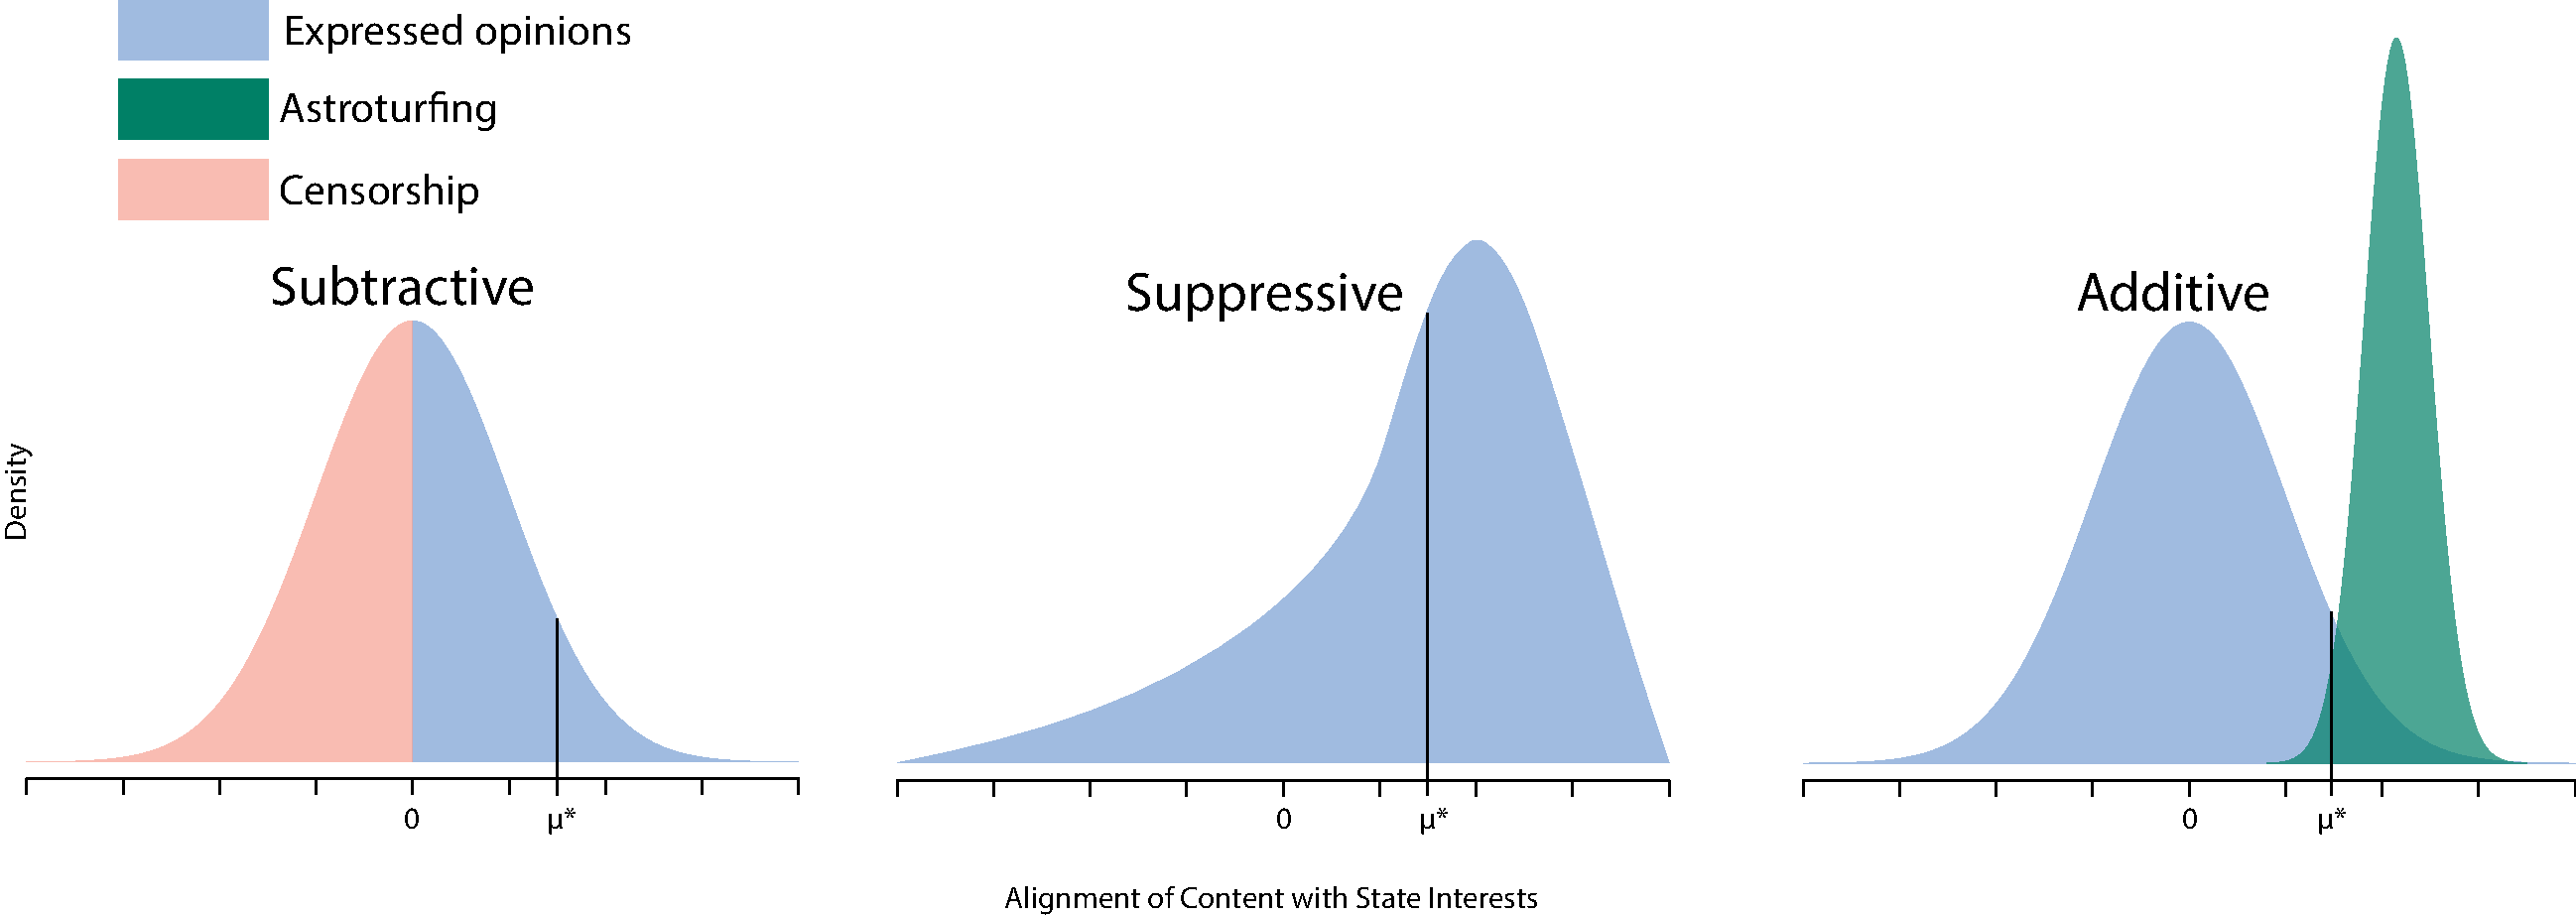
\includegraphics[width=\textwidth]{figures/info_manip_dist.pdf}\\
      \scriptsize{\it If the true density of opinions held by individuals in society is assumed to be symmetric around neutral viewpoint (zero), each of the three plots is an illustration of how each of three major information manipulation tactics can move the visible and expressed opinions toward the state's ideal, $\mu_{+}$.}\vspace{2em}
      \label{info_manip_dist}
    \end{center}
\end{minipage}

These three types of information control can also vary in their conspicuousness. In additive information manipulation, the identity of the state as the information manipulator is sometimes present and sometimes obscured. In some circumstances, government bureaucrats participate in online discourse openly with the identity of a bureaucrat (i.e. their name and title are visible in their social media profile, they wear a uniform in their profile picture, or are posting from an official government account). In other circumstances, the bureaucrat will deliberately obscure her identity to appear like she is an ordinary citizen. Each type of information control in \hyperref[info_manip_dist]{Figure \ref*{info_manip_dist}} has overt and covert forms.

Of course, each of these tactics themselves differ in the degree to which the information manipulation is observed and the degree to which the identity of the information manipulator is identifiable. Subtractive information manipulation, for example can only be overt or covert if the deletion of content is reported to the user, which in some cases it is. In most cases, comments are deleted without notice to the user. Suppressive and additive information control are more conspicuous in both overt and covert forms than most subtractive information. Because suppressive information control seeks to dissuade individuals from posting anti-regime messages using carrots and sticks, the information control tactic is almost always observed. In additive information control, the information control tactic can be observed in overt form if the resulting distribution of opinions is so skewed that it does not seem plausible to the user. In overt forms, the presence of opinions from state-affiliated individuals means this information control tactic is observed.

\section{Survey Experiments}

I examine the effectiveness of additive, subtractive, and suppressive information control tactics using three survey experiments. A covert and overt version of each of the three aforementioned types of information control are randomly assigned to users on a custom-built news website that records behavioral analytics data: clicks of comment likes, dislikes, and reports, as well as the subjects own comments. In each experiment, I compare the effectiveness of each of the three information control tactics in their overt and covert forms. In all experiments, subjects answer identical pre-treatment and post-treatment questionnaires. Pre-treatment questions include demographic questions: age, gender, income, ethnicity, education, location, work unit, hukou (see \hyperref[pre_treatment]{Table \ref*{pre_treatment}} in the appendix). Subjects are asked to self-report their media exposure by asking them the variety of outlets and programs they are exposed to in print media, online media, social media, and television as well as the extent to which they consume these media (see \hyperref[exposure]{Table \ref*{exposure}} in the appendix for the media sources asked about). Subjects are also asked several questions to measure political knowledge. Several covertly-placed questions measure government support.

Post-treatment questions measure the effectiveness of information control, the impact of information control on user experience, the perceptions of discourse competition, and perceptions of how representative comments in the comment section are to opinions held by the public (see \hyperref[types_info_control]{Table \ref*{types_info_control}}). The full text of these questions can be found in \hyperref[post_treatment_1]{Table \ref*{post_treatment_1}} and \hyperref[post_treatment_2]{Table \ref*{post_treatment_2}} in the appendix.

In all three experiments, subjects are sent to a website outside of the Qualtrics survey interface to perform ``user testing'' of a new design for a fictional news website, ``Now News.'' The user testing interface loads in a new window when clicked from the Qualtrics survey. This user testing interface displays instructions at the top of the page. In the instructions, subjects are directed to ``read the article, like or dislike comments in the comment section, and leave [their] own comment if [they] would like to.'' They are told that they will need to pay attention to the content of the article and its comments to complete the next round of survey questions. They are reminded of this in a pop-up modal when they scroll down to the comments section.

Below these instructions, a ``live version'' of the news site dynamically loads in a large frame. A loading screen is displayed to lead the subject to believe they are being redirected to an external website.\footnote{The news site is modeled after the mobile version of the Sina News and the Associated Press websites.} The news site that loads is comprised of a news article and its comment section. See the text of the article in \hyperref[text]{Section \ref*{text}} and screenshots of the vignettes in \hyperref[interface]{Section \ref*{interface}} in the appendix). In all experiments, the user testing interface contains a summarized Global Times op-ed about a new government ride sharing policy. I chose a Global Times article on ride sharing services for the vignette because of the topic's salience, lack of political sensitivity, and the presence of an active online debate on the topic. The article was summarized by a research assistant and checked for errors and believability by two other research assistants, all of whom are native speakers. As Global Times is a state media outlet, the op-ed champions the new policy.

Subjects are advised that the article's comment section is live, with ``actual user comments, posted in real time.'' When they have finished interacting with the article, they continue to post-treatment questions. Comments displayed below the article are selected from the real comment sections of a variety of outlets that have syndicated the original editorial in order to make the experience as realistic and externally valid as possible. Each comment has been categorized according to its polarity in support or opposition of the ride sharing policy. The distribution of the polarity of comments varies across treatment groups, as do the identities of the comments' respective authors. Comments can be liked, disliked, or reported, and these user interactions are saved in a database to be used as behavioral outcomes. The position of the comments in the comment section have been randomly ordered on the page, so that the position of comments of different polarity will not affect the outcome. The comment text, each comment's polarity, and each comment's position can be found in \hyperref[comments]{Table \ref*{comments}} in the appendix. Subjects can also leave their own comments which appear dynamically in the comment section and are saved in the database as an additional behavioral outcome.

\subsection{Experiment 1: Effectiveness of Additive Information Control}\label{exp:1}

The first experiment tests if and how additive information in overt and covert forms can be effective. More specifically, it examines the effectiveness of comment propaganda and astroturfing. Comment propaganda, an overt information control tactic, is commonly deployed across social media platforms in China by bureaucracies and select government officials who are encouraged to cultivate an online presence and serve as opinion leaders. Astroturfing, a covert form of comment propaganda, is also commonly deployed by bureaucrats across China in an effort to increase the apparent mass support for the Party, local government, and their respective policies. Astroturfing, named after a brand of artificial turf, refers to the intended effect of this information control tactic: to fake grassroots support.

The experiment has 2 treatment groups and one control. The control displays 9 comments that are balanced according to their polarity: 3 pro-ride sharing policy comments, 3 neutral comments, and 3 anti-ride sharing policy (see \hyperref[baseline]{Figure \ref*{baseline}} in the Appendix for a screenshot of the comment section). This control group is the same across all three experiments. In overt and covert treatments, an additional 6 pro-ride sharing policy comments are displayed to the user. These 6 comments have been randomly distributed among the 9 comments in the baseline condition. In the covert treatment, the identities of these additional pro-ride share policy comments (their profile picture and their account name) resemble ordinary people (see \hyperref[CA]{Figure \ref*{CA}} in the Appendix for a screenshot of the comment section). In the overt treatment, they resemble government bureaucracies or bureaucrats  (see \hyperref[OA]{Figure \ref*{OA}} in the Appendix for a screenshot of the comment section). The identities of the users in the comment sections are fictional, but based on real user profiles from the Sina News and Sina Weibo platforms. A table of the overt and covert user identities can be found in \hyperref[uids]{Table \ref*{uids}} and \hyperref[uidgov]{Table \ref*{uidgov}} in the appendix.

\subsection{Experiment 2: Effectiveness of Subtractive Information Control}

The second experiment tests if and how subtractive information in overt and covert forms can be effective. Subtractive information---removal of information from public view---is closest conceptually to what most would associate with ``censorship.'' Many different tactics, however, fit underneath the umbrella of censorship. In China, users are sometimes notified when content is censored, but increasingly content is removed without the original author of content or her audience's knowledge. In recent years, many platforms have stopped displaying censorship notifications to users, ostensibly because these notices are unpleasant and negatively affect user experience. To the author's knowledge, there have yet to be any studies to identify the effects of covert subtractive information control on opinion and behavior. Treatments in this experiment simulate how users experience overt and covert and overt forms of subtractive information control. In the two treatment groups, negative comments are removed from the comment section, leaving the 3 neutral and 3 positive comments. These treatments are compared to the same control group discussed in \hyperref[exp:1]{Section \ref{exp:1}}.

For the overt condition (see \hyperref[OS]{Figure \ref*{OS}} in the Appendix for a screenshot of the comment section), a notice at the top of the comment section reads:

``Some comments may relate to content that does not comply with relevant laws, regulations, and policies, and have not been displayed.''

For covert subtractive condition, no such notice is displayed (see \hyperref[CS]{Figure \ref*{CS}} in the Appendix for a screenshot of the comment section). In both treatment conditions, the number of comments is displayed (9 comments) with an additional notice in parentheses that reads, ``3 comments not shown.''

\subsection{Experiment 3: Effectiveness of Suppressive Information Control}

This experiment tests if and how suppressive information in overt and covert forms can be effective. In particular, this experiment examines how notifying users that they are under surveillance can affect opinion and behavior. On various social media platforms, it is common to subtly suggest that social platforms are moderated to encourage more civil and less disruptive behavior on the platform. Sometimes this involves a notice of regulations for commenting on the platform. Other times, such a prompt overtly references government regulations. These messages, though subtle, are repressive. They are meant to signal surveillance, induce fear, or depress political expression. For these suppressive treatments, users are given a notice of comment moderation at the top of the comment section. These treatments are compared to the same control group discussed in \hyperref[exp:1]{Section \ref{exp:1}}.

For the overt treatment (see \hyperref[OSP]{Figure \ref*{OSP}} in the Appendix for a screenshot of the comment section), users are presented with a small cartoon of an internet police officer above the comment section along with the following notice:

``In order to protect the safety and quality experience of our users, this platform is supervised by internet police.''

For the covert treatment (see \hyperref[CSP]{Figure \ref*{CSP}} in the Appendix for a screenshot of the comment section), users are presented with the Now News logo and the following notice:

``In order to protect the safety and quality experience of our users, this platform is supervised by our staff.''

\subsection{Post-treatment Measures}

After subjects interact with the web testing interface, they are directed back to the survey to answer a battery of questions measuring the effectiveness of these information control tactics. Because the academic literature offers many explanations for why censorship, propaganda, and repression are effective, there has yet to be a study adjudicating between these explanations experimentally in a realistic online environment.

This pre-analysis plan will preregister hypotheses about the relative effectiveness of covert and overt tactics, but the study will also seek to adjudicate between various explanations for {\it how} each tactic will and will not be effective. This part of the design is more inductive---there is little existing evidence to support hypotheses for exactly how these different tactics will be effective.

In the next section I will detail the theoretical support for how information control tactics might be effective and hypothesize how and why covert tactics will outperform overt tactics.

\section{Theory and Empirical Expectations}

The state and media companies share a common interest in making information control tactics less visible and less invasive to users. Media companies want to at least maintain, and ideally increase user engagement over time. The state is also aware that heavy handed information control tactics can backfire. Media companies are well-equipped to prevent negative experiences that can lead to backfire because they have expertise the state does not: their success depends on their ability to affect change in user behavior (i.e. through advertisements) and the state does not have the data or experience to achieve this goal.

Because of a shared interest in increasing engagement and minimizing disruptions to users, private companies and the state have reached an equilibrium over the past several years: the use of covert information control tactics. Because repression and intimidation often backfire, the state and social media companies have adapted information control to involve mostly gradual and covert measures to ``channel'' and ``guide'' public opinion \citep{roberts2018censored,roberts2017censorship}. I argue that information control is most effective when those who experience information control tactics cannot readily perceive them and thus believe that the information they consume is representative of the views of society at large.

Perceptions of discourse competition and covertness are key to the effectiveness of information control tactics. Discourse competition represents the degree to which different points of view can be expressed and contested. In an online forum, discourse competition is a signal of whether the information they consume is a representative sample of opinions held by the public. Similarly, covertness of information control tactics---how visible it is to information consumers that the information they observe has been manipulated or curated---can also be a signal of whether the information they consume is a representative sample of opinions held by the public.

Much of the literature on how consumption of information can affect opinion and behavior focuses on information consumed in the aggregate. In Zaller's seminal work on opinion formation, individuals receive information from the media and their social interactions \citep{zaller1992nature}. Their opinion formation is contingent on the information to which they are exposed, the subset of that information they choose to accept, and the information they later sample from their memory. In this analysis I focus on a key part of this model: what will cause individuals to {\it accept} information they {\it receive}. I argue that perceptions of discourse competition and the degree to which information has been manipulated affects whether the individual chooses to accept that information as reliable, reputable, and/or true. If a government seeks to guide public opinion, they could constrain the maximization of visible favorable opinions---taking care not to reduce perceptions of discourse competition or make their interventions overt. Those who observe this distribution of opinions that is more favorable to the government might infer greater support or social desirability of pro-government opinions.

In other words, if the state is mindful of how it perturbs the distribution of opinions that individuals {\it receive}, it can influence what individuals are likely to {\it accept}. Take for example an individual who holds an anti-government opinion. If they are presented with a sample of opinions from their peers that seems credible and unadulterated, but nonetheless has been deliberately perturbed to over-represent pro-government opinions, they could be persuaded that their own opinion is unpopular, even if it is in fact a popular opinion. If this individuals' opinion is weakly held, they might even update it out of concern for social desirability. If, however, the state is observed as the information manipulator, the distribution of opinions the individual receives will be seen as unrepresentative of the opinions held by their peers. I hypothesize that covert information interventions will be more effective than overt ones because a sample of opinions that appear to be manipulated by the state will be seen as less representative of the opinions of ones peers than a sample of opinions that appears unperturbed.

\subsection{Effectiveness}

In this analysis, I measure the effects of three common types of information control---additive, subtractive, and suppressive---on measures of opinion and behavior that correspond to regime goals. Suppressive information control refers to repressive/cooptative measures to suppress expression, and is usually targeted at individuals who are influential and often produce anti-regime content \citep{gallagher2019who,roberts2018censored}. This tactic is carried out either by the state or its agents (often private companies). When carried out by the state, suppressive information control is more overt because the state's role in this information control intervention is clear. When carried out by private companies, the state's role is obscured and more covert. I expect suppressive information control will be effective at decreasing self-expression and willingness to participate in collective action because it will trigger fear of social costs or repression when experienced. Additive and subtractive information control tactics, by contrast will more effectively impact attitudes and support for the government and its policies. This is because these tactics add or remove content, altering the distribution of visible opinions from which subjects will sample to form their opinions. Because these tactics alter the distribution of visible opinions, they will impact perceptions of discourse competition more than the suppressive information control treatment. 

A typology of discourse competition (low, high) and the conspicuousness of the information manipulator's true identity is illustrated in \hyperref[types_info_control]{Table \ref*{types_info_control}}. Each of the cells in this typology refer to a treatment group in the three experiments detailed in the previous section.


An ``effective'' information intervention is one that contributes positively to the state's broad goals of solidifying legitimacy, increasing regime support, preventing spontaneous collective action, and/or mobilizing nationalist sentiment. The expected direction of each outcomes measure if the information control tactic is effective can be found in \hyperref[hypotheses_info_control]{Table \ref*{hypotheses_info_control}}. The theoretical support and measurement strategy for each variable is described in detail below. I measure each variable using survey scales, open-ended questions, and behavioral analytics. Open-ended questions are coded according to diagrams in \hyperref[diags]{Section \ref*{diags}} in the appendix. Some variables are measured using behavioral analytics gathered from interactions with the treatment vignette website.

\begin{table}[h]
    \centering
    \caption{Types of Information Control}
    \label{types_info_control}
        \begin{tabular}{|c|c|c|c|c|c|c|}
            \cline{3-4}
            \multicolumn{2}{p{.01\textwidth}p{.01\textwidth}|}{} & \multicolumn{2}{c|}{Discourse Competition}  \\ \cline{3-4}
            \multicolumn{2}{p{.01\textwidth}p{.01\textwidth}|}{} & Low & High \\ \hline
            \multirow{2}{*}{Conspicuousness} & Low & Covert Subtractive (CSB) & Covert Additive (CA) \\  \cline{2-4}
            & High & Overt Subtractive (OS) & Overt Additive (OA) \\ \hline
        \end{tabular}
\end{table}

I expect that information control tactics will be more effective in covert forms. More specifically, subjects will be more likely to {\it accept} pro-government messages when they think the author is a peer or when they think content moderators are disinterested and unaffiliated with the government.\newline

\noindent\underline{Hypothesis 1:} Information interventions will be more effective in covert forms.\newline

\begin{table}[H]
    \centering
    \caption{Effectiveness Outcome Measures; Expected Direction if Effective}
    \label{hypotheses_info_control}
    \resizebox{\textwidth}{!}{
        \begin{tabular}{|l|c|c|c|c|c|}
        \hline
        \textbf{Variable} & \textbf{Expected Direction} & \textbf{Survey Scale(s)} & \textbf{Open Ended} & \textbf{Behavioral (Y/N)} \\ \hline
            Support of Policy & +  & Q32 & Q30 & Y \\ \hline
            Unpopularity of Opinion (Pro) & - & Q31, Q32 & & N \\ \hline
            Unpopularity of Opinion (Anti) & + &  Q31, Q32 & & N \\ \hline
            Legitimacy & + & Q42, Q43 & Q44 & N \\ \hline
            Trust in State Media & + & Q39, Q40 & Q41 & N \\ \hline
            Nationalism & + & Q50 & Q51 & N \\ \hline
            Favorable Comments & + & & & Y \\ \hline
            Unfavorable Comments & - & & & Y \\ \hline
            User Satisfaction & - & Q50 & Q51 & N \\ \hline
            Self-Expression (Regime Supporter) & + & Q33, Q34 & & Y \\ \hline
            Self-Expression (Regime Opponent) & - & Q33, Q34 & & Y \\ \hline
            Collective Action & - & Q53, Q54, Q55 & Q56 & N \\ \hline
        \end{tabular}
    }
\end{table}

%\begin{table}[H]
%    \centering
%    \caption{Representativeness and Discourse Competition}
%    \label{hypotheses_info_control}
%        \begin{tabular}{|l|c|c|c|}
%        \hline
%        \textbf{Variable} & \textbf{Survey Scale(s)} & \textbf{Open Ended} \\ \hline
%            Representativeness & Q35 & Q37 \\ \hline
%            Discourse Competition & Q36 & Q37 \\ \hline
%        \end{tabular}
%\end{table}

In the following subsections, I discuss each way that information control can be effective. In each section, I cite relevant literature, discuss the design of survey scales, open-ended questions and the coding procedure for each, and behavioral measures of effectiveness (if applicable).

\subsubsection{Agreement with Policy}

The first measure of effectiveness is level of agreement with the ride-share policy. An effective intervention will increase agreement with the rideshare policy discussed in the article.

Though measuring a sustained change in opinion is difficult in a one-off experiment, agreement with the rideshare policy described in the article can proxy for effective ``opinion guidance.'' The Chinese state ``guides opinion'' by increasing the visibility of pro-regime messages and decreasing the visibility of anti-regime messages. The state can guide opinion through sustained propaganda campaigns \citep{geddes1989sources}. But it can also suppress negative opinions by encouraging people to act ``as if'' they support the regime through their behavior and expression even if their attitudes remain unchanged \citep{wedeen1999ambiguities}. Pro-regime ``cheerleading'' or promotion of ``positive energy'' in online forums may accomplish this through distraction \citep{king2016chinese} or increasing `` information friction'' \citep{roberts2018censored}.

I measure how effectively each information control tactic ``guides opinion'' by asking respondents how much they support or oppose the ride-share policy described in the article. To measure how popular they believe their own opinion is, respondents are also asked to provide an assessment of how much their peers agree or disagree with the ride-share policy. This allows examination of how additive and subtractive information control tactics increase or decrease the perceptions of popular support for one opinion over another. An effective information control tactic will increase support for the rideshare policy.

Using identical scales, I ask subjects {\it their own} opinion and their perception of {\it peers'} opinion on the rideshare policy. To measure how subjects perceive the popularity or social desirability of their opinion, I record the distance between their level of agreement with the rideshare policy and their peers' level of agreement with the rideshare policy. An effective information control tactic will increase this distance for opponents (make opponents think their opinion is unpopular) and decrease this distance for supporters (make supporters think their opinion is popular).

In addition to direct survey scales, subjects are asked an open-ended question (see Q30 in \hyperref[post_treatment_1]{Figure \ref*{post_treatment_1}} in the Appendix) asking them to share their opinion about the new ride share policy and are given the option of leaving a comment in the comment section. Their agreement with the rideshare policy will be measured according to a positive (1), neutral (0), or negative (-1) valence scale for both of these data points according to the ``favorability'' coding diagram in \hyperref[favorability]{Figure \ref*{favorability}} in the Appendix.

To mitigate problems with reliability of self-reported opinions, an alternative measure of agreement with the policy makes use of behavioral analytics that track clicks of ``like'' and ``dislike'' buttons for each comment in the comment section. In each experiment, support for the policy is measured as follows:
$$(\text{pro-govt. likes } + \text{ anti-govt. dislikes}) \,-\, (\text{pro-govt. dislikes } + \text{ anti-govt. likes})$$

\subsubsection{Self-Expression}

The second measure of effectiveness is ``self-expression.'' An effective intervention will 1) increase the expression of government supporters and decrease the expression of government opponents or 2) increase the expression of favorable comments and decrease the expression of unfavorable comments.

Past work on how individuals experience censorship have shown that experiencing censorship can have counter-intuitive effects. \cite{roberts2015experiencing} found that experiencing censorship {\it increased} unfavorable expression because it made individuals angry. \cite{hobbs2016sudden} similarly find that censorship can backlash, prompting individuals to seek out information and censorship circumvention technology---eventually leading to greater access to unfavorable information. In this analysis, I will examine how different kinds of information control might increase or decrease the expression of regime supporters and opponents {\it as well as} the expression of negative and positive information. 

First, I measure self-expression using survey scales targeting willingness to express opinion, behavioral measures such as the length of open-ended text responses, the count of comments on the article made by subjects, and the count of interactions made on the website (all likes, dislikes, and reports). To show the effect of expression conditional on regime-support, I will look at treatment-by-covariate interaction effects with a regime support scale.

I customized this regime support scale for this project and drew inspiration from the ``diffuse support scale'' used in \cite{wang2018corruption} and the scales for trust in government used in the Beijing Area Survey (BAS). My scale is more covertly worded in order to mitigate the very high dropout seen in pilot studies when using the ``diffuse support scale.'' These questions measure trust in local and central government leaders, past party/state employment affiliation, the media consumption ratio of official media sources to semi-official or commercialized sources, the ability to correctly attribute political slogans to Xi Jinping, and if they have downloaded the propaganda app, {\it xuexi qiangguo}. Using these manifest variables, I will construct a latent variable using IRT.

Second, I look at expression of negative- and positive-valence comments. Effective information control tactics may also decrease the willingness of an individual to express an favorable opinion and increase the willingness to express an unfavorable opinion.

The valence of comments will be coded using the same ``favorability'' coding diagram in \hyperref[favorability]{Figure \ref*{favorability}} in the Appendix. Additionally, valence of expression is measured using behavioral analytics from the vignette website---the count of comments and likes by the respondent and the coded text of open-ended responses and comments. Favorable expression and unfavorable expression will be operationalized as the count of favorable comments and the count of unfavorable comments respectively.

\subsubsection{Solidifying Perceptions of Legitimacy}

The third measure of effectiveness is ``legitimacy.'' An effective intervention will increase perceptions of the state's {\it performance legitimacy} or {\it moral/legal authority}.

Preserving and bolstering legitimacy is a common goal of all regimes. \cite{huang2014propaganda} finds that though the messages in state propaganda are not persuasive, they signal legitimacy, benevolence, and capacity. To examine the effect of each type of information control on perceptions of regime legitimacy, respondents are asked questions targeting two main sources of legitimacy in authoritarian regimes: robust and continued economic performance, sometimes referred to as ``performance legitimacy'' \citep{bueno2005development, zhao2009mandate}, and the state's moral authority \citep{ding2019justice,grzymala2015nations}. More specifically, questions ask whether respondents believe the government is serving the people and responding to their needs, and a question targeting ``performance legitimacy,'' which broadly asks their satisfaction with the status quo in China.

An information control tactic that is effective at increasing perceptions of legitimacy will increase satisfaction with the status quo and increase subjects' belief that the government is serving the people and responding to their needs. I measure this using survey scales asking each of these questions directly and an open-ended follow-up asking them to explain their answers. This open-ended survey response will be coded into a positive (1), neutral (0), or negative (-1) valence scale for both of these data points according to the ``legitimacy'' coding diagram in \hyperref[legitimacy]{Figure \ref*{legitimacy}} in the Appendix.

\subsubsection{Preventing Spontaneous Collective Action}

The fourth measure of effectiveness is ``collective action.'' An effective intervention will decrease willingness of individuals to engage in collective action.

\cite{huang2014propaganda} finds that propaganda can decrease the willingness of individuals to participate in collective action. \cite{king2013censorship,king2014reverse} also argue that preventing collective action is a central goal of government information control.

To examine the effect of each type of information control on willingness to engage in collective action, respondents are asked whether they would be willing to sign a petition,  join a march, or formally petition (\zh{信访、上访}) in favor of a strongly held opinion or conviction. An information control tactic that is effective at decreasing collective action will decrease willingness to engage in these behaviors.

I ask subjects to explain their responses to these survey scales in an open-ended question. This way I can better understand their reasoning for willingness/unwillingness to engage in collective action. These responses are coded using the ``collective action'' coding diagram in \hyperref[collective_action]{Figure \ref*{collective_action}} in the Appendix. Of particular interest is the subcategory ``fear'' which may provide suggestive evidence that fear is a causal mechanism behind a decrease in willingness to engage in collective action. Unfortunately, this relies on the respondent's willingness to share their fear, so it might not be possible to test this mechanism. Asking the respondent directly about their fear is likely to be unreliable or cause undue attrition.

\subsubsection{Mobilizing Nationalist Sentiment}

The fourth measure of effectiveness is ``nationalism.'' An effective intervention will increase nationalist sentiment. In certain circumstances (during times of domestic/foreign conflicts) it can be in the regime's best interest to mobilize nationalist sentiment. To measure nationalist sentiment, I use a scale from the Beijing Area Survey (BAS). This question targets three components of nationalism: pride in and valuation of the nation, ethnocentrism, and blind/na\"{\i}ve support for the nation-state \citep{johnston2017chinese}.

In addition to this survey scale, I ask subjects to explain their responses in an open-ended question, this will serve as an additional measure of nationalism and allow for more rich qualitative analysis of how each of the information control treatments are affecting nationalist sentiment.

\subsubsection{Trust in State Media}

The fifth and final measure of effectiveness is ``trust in state media.'' An effective intervention will increase or maintain levels of trust in state media.

While some have explored how political trust and media effects affect one another \citep{chen2001media,cai2018media}, and others have explored backlash resulting from ``hard propaganda'' \citep{huang2014propaganda, huang2016media}, reputational costs incurred by state media when users experience information control remain underexplored.

To measure trust in state media, I ask users two questions. The first is about the trustworthiness of {\it Xinwen Lianbo}, the nightly state media broadcast with the highest perceived affiliation with the ruling Communist Party. To measure relative trustworthiness of news by source, I use a scale from the 2017 "Netizen Readership and Attitude Survey" whose results are published in the ``Political Participation Blue Book'' \citep{ma2017zhengzhi}. This scale asks how trustworthy users would find a variety of sources if they were looking for information about a sudden incident like a government corruption scandal.

In addition to this survey scale, I ask subjects to explain their responses in an open-ended question, this will serve as an additional measure of media trust and allow for richer analysis of what how---if at all---information control treatments are affecting trust in state media.

\noindent\underline{Hypothesis 2:} Overt information control and information control with low perceived discourse competition will decrease trust in state media.\newline

\subsection{Perceived Discourse Competition and ``Representativeness'' of Comments}

In authoritarian regimes that monopolize or heavily regulate media, citizens are aware that information they consume does not come from objective and disinterested sources. Many authoritarian regimes, however, have semi-commercialized media, which results in a perception that some media outlets are more independent than others \citep{stockmann2013media}. Just as competitiveness at the source level can increase the credibility of information to consumers, opening circumscribed spaces for contentious discourse on a micro-scale can counter-intuitively increase the credibility of pro-regime information. \cite{han2018contesting} argues that the state benefits from contestation online because individuals are distrustful of the intentions of those espousing anti-regime opinions, not because they are convinced by state propaganda. The presence of pro-government information and anti-government information suggests that there is some discourse competition, and that the distribution of opinions in these forums may be unadulterated and representative of the opinions held by society at large.

Because the distribution of opinions resulting from subtractive interventions result in no anti-regime viewpoints, there is less discourse competition, and observed opinions are less likely to be seen as unadulterated or credible representations of the opinions of ones peers. The level of discourse competition should affect how users accept the information they consume in the comments.

\noindent\underline{Hypothesis 3a:} Individuals will perceive that the comment sections in the additive information control treatment groups are more representative of the opinions held by ordinary citizens than comment sections in the subtractive information control treatment groups.\newline
\noindent\underline{Hypothesis 3b:} Individuals will perceive that there is more discourse competition in the comment sections in the additive information control treatment groups than comment sections in the subtractive information control treatment groups.\newline

Information in online forums will be perceived as more credible if commentators are perceived as ordinary citizens or if content moderators are perceived as disinterested and impartial. Self-assessments are rarely if ever impartial. People tend to treat them with skepticism or ignore them entirely. A restaurant's claims that they are ``the best in town'' is not nearly as credible as the same claim from a friend or peer. This is why restaurants, companies, and governments engage in online astroturfing.\newline

\noindent\underline{Hypothesis 4a:} Individuals will perceive that the comment sections in the covert information control treatment groups are more representative of the opinions held by ordinary citizens than the comment sections in the respective overt information control treatment groups.
\noindent\underline{Hypothesis 4b:} Individuals will perceive that there is more discourse competition in the comment sections in the covert information control treatment groups than the comment sections in the respective overt information control treatment groups.

\subsection{User Satisfaction}

Covert censorship minimizes the anger and backlash that \cite{roberts2018censored} finds results from experiencing censorship. This backlash is bad for both private internet platforms and the state. By preventing backlash, covert censorship also reduces the occurrence of conflicts between users and the state over the acceptable bounds of discussion.\newline

\noindent\underline{Hypothesis 5:} Overt information control tactics will decrease user satisfaction more than covert information control tactics.

\subsection{Mediation Effects}

I hypothesize that the degree of perceived discourse competition mediates the effectiveness of information control tactics. To test this mediation effect, I will run a causal mediation analysis with a scale for discourse competition as the mediator. This scale for discourse competition will be constructed using IRT and will include four questions asking about discourse competition in the comment section.\\

\noindent\underline{Hypothesis 6:} Perceptions of discourse competition will mediate the effectiveness of information control.

\subsection{Heterogeneous Effects}

Several pre-treatment variables test common interactions found in the media effects literature. Each is detailed below:

\subsubsection{Media Exposure}

I measure media exposure with survey questions similar to those in \cite{stockmann2013media}. She finds that media effects are conditional on the type of media sources to which individuals are exposed. These media exposure measures are used to test for heterogeneous effects of media exposure on the various ``effectiveness'' outcomes described in detail below. Using the same typology of ``official,'' ``semi-official,'' and ``commercialized'' used by \cite{stockmann2013media}, I present disaggregated measures of media exposure by source type in addition to the aggregate measure.\newline

\noindent\underline{Hypothesis 7a  (Persuasion):} Persuasion effects will be larger at lower levels of media exposure.\\
\noindent\underline{Hypothesis 7b  (Persuasion):} Persuasion effects will be larger at lower levels of media exposure.\\
\noindent\underline{Hypothesis 7c  (Persuasion):} Persuasion effects will be larger at lower levels of media exposure.

\subsubsection{Political Knowledge}

I measure political knowledge using a battery of six questions that ask subjects to answer questions about China's political system, its leaders, and historical political events. Each question has a correct and incorrect answer and the questions vary in difficulty. An aggregate measure of political knowledge is calculated using IRT of each binary indicator for a correct answer.\newline

\noindent\underline{Hypothesis 8a  (Persuasion):} Persuasion effects will be larger at lower levels of political knowledge.\\
\noindent\underline{Hypothesis 8b  (Trust in state media):} Trust in state media effects will be larger at lower levels of political knowledge.\\
\noindent\underline{Hypothesis 8c  (Legitimacy):} Legitimacy effects will be larger at lower levels of political knowledge.

\subsubsection{Regime Support}

I measure regime support using several questions that unobtrusively ask for regime support. The questions that form this scale include support for local and central government leaders, past party/state employment affiliation, the media consumption ratio of official media sources to semi-official or commercialized sources, the ability to correctly attribute political slogans to Xi Jinping, and if they have downloaded the propaganda app, {\it xuexi qiangguo}. I estimate a latent measure of regime support using IRT of each of these questions.\newline

\noindent\underline{Hypothesis 9a  (Persuasion):} Persuasion effects will be larger as regime support increases.\\
\noindent\underline{Hypothesis 9b  (Trust in state media):} Trust in state media effects will be larger as regime support increases.\\
\noindent\underline{Hypothesis 9c  (Legitimacy):} Legitimacy effects will be larger as regime support increases.

\subsubsection{Censorship Circumventer}

In the block of questions about media exposure, I ask individuals to self report exposure to news sources and social media platforms that are blocked in mainland China (such as the New York Times and Facebook). Self-reported exposure to these sources suggests that the subject either circumvents internet censorship or is abroad frequently enough to access these websites on a monthly basis.\newline

\noindent\underline{Hypothesis 10a  (Persuasion):} Persuasion effects will be smaller for subjects who circumvent internet censorship.\\
\noindent\underline{Hypothesis 10b  (Trust in state media):} Trust in state media effects will be smaller for subjects who circumvent internet censorship.\\
\noindent\underline{Hypothesis 10c  (Legitimacy):} Legitimacy effects will be smaller for subjects who circumvent internet censorship.

\section{Results}

Additive and subtractive information control conditions significantly decreased subjects perceptions of discourse competition in the comment section (see \hyperref[ATE_discourse_comp]{Figure \ref*{ATE_discourse_comp}}).

\vspace{-2em}
\begin{minipage}{\linewidth}
    \begin{center}
  		\captionof{figure}{Perceptions of Discourse Competition by Treatment Group}
        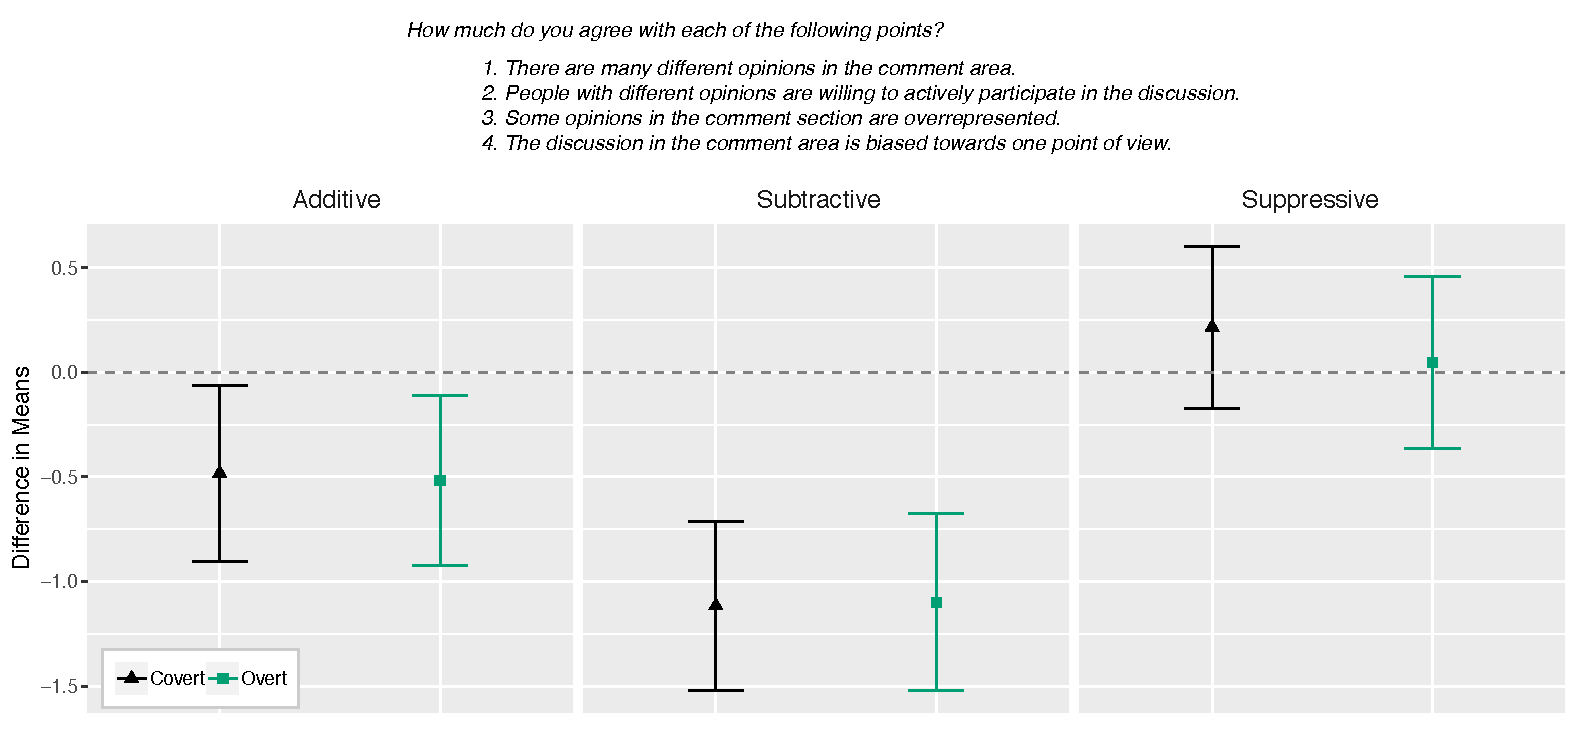
\includegraphics[width=.9\textwidth]{figures/ATE_discourse_comp.pdf}\\
        \label{ATE_discourse_comp}
    \end{center}
    \vspace{.5em}
\end{minipage}

Contrary to expectations, however, I did not find evidence that perceptions of discourse competition increased or decreased the effectiveness of information control, there were no statistically detectable difference between {\it overt} and {\it covert} treatment groups across all measures of effectiveness.

Additionally, subtractive information control was effective across many different measures, while additive information control was not effective by any measure. Subtractive information control increased agreement with the rideshare policy, decreased expression, increased nationalist sentiment, and increased perceptions of legitimacy (but only in the covert treatment), and media trust (but only in the covert treatment). In these last two outcomes, though the difference in the magnitude of coefficients is in the right direction ({\it covert} information control is more effective than {\it overt} information control), they are not statistically distinguishable from one another.

\begin{minipage}{\linewidth}
    \vspace{.5em}
    \begin{center}
  		\captionof{figure}{Agreement with the Rideshare Policy by Treatment Group}
        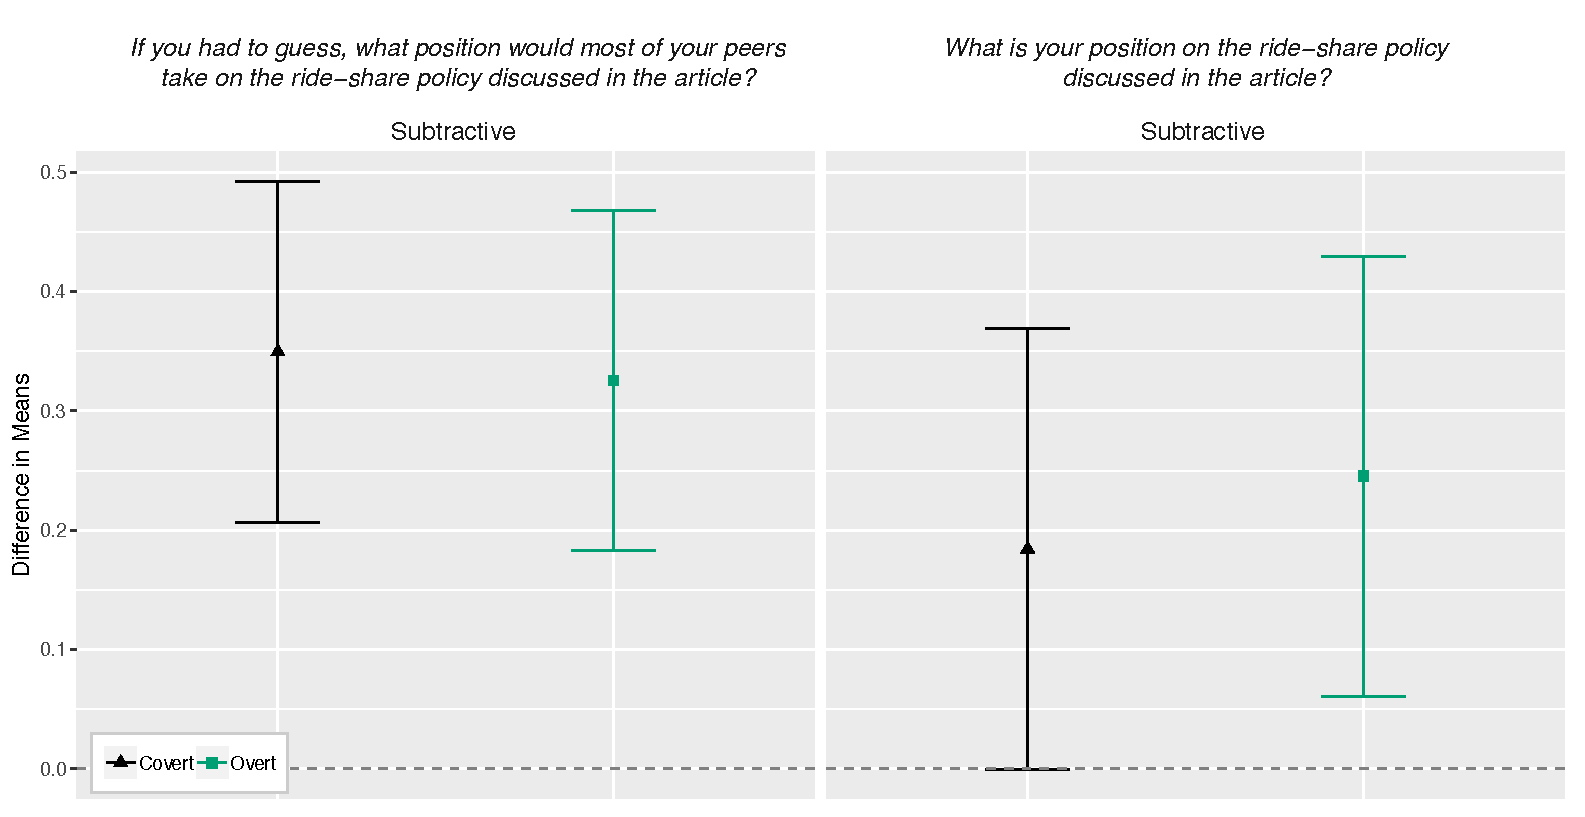
\includegraphics[width=.9\textwidth]{figures/ATE_opinion.pdf}\\
        \label{ATE_opinion}
    \end{center}
\end{minipage}

\begin{minipage}{\linewidth}
    \vspace{1em}
    \begin{center}
  		\captionof{figure}{Expression Measures for the Subtractive Treatment Group}
        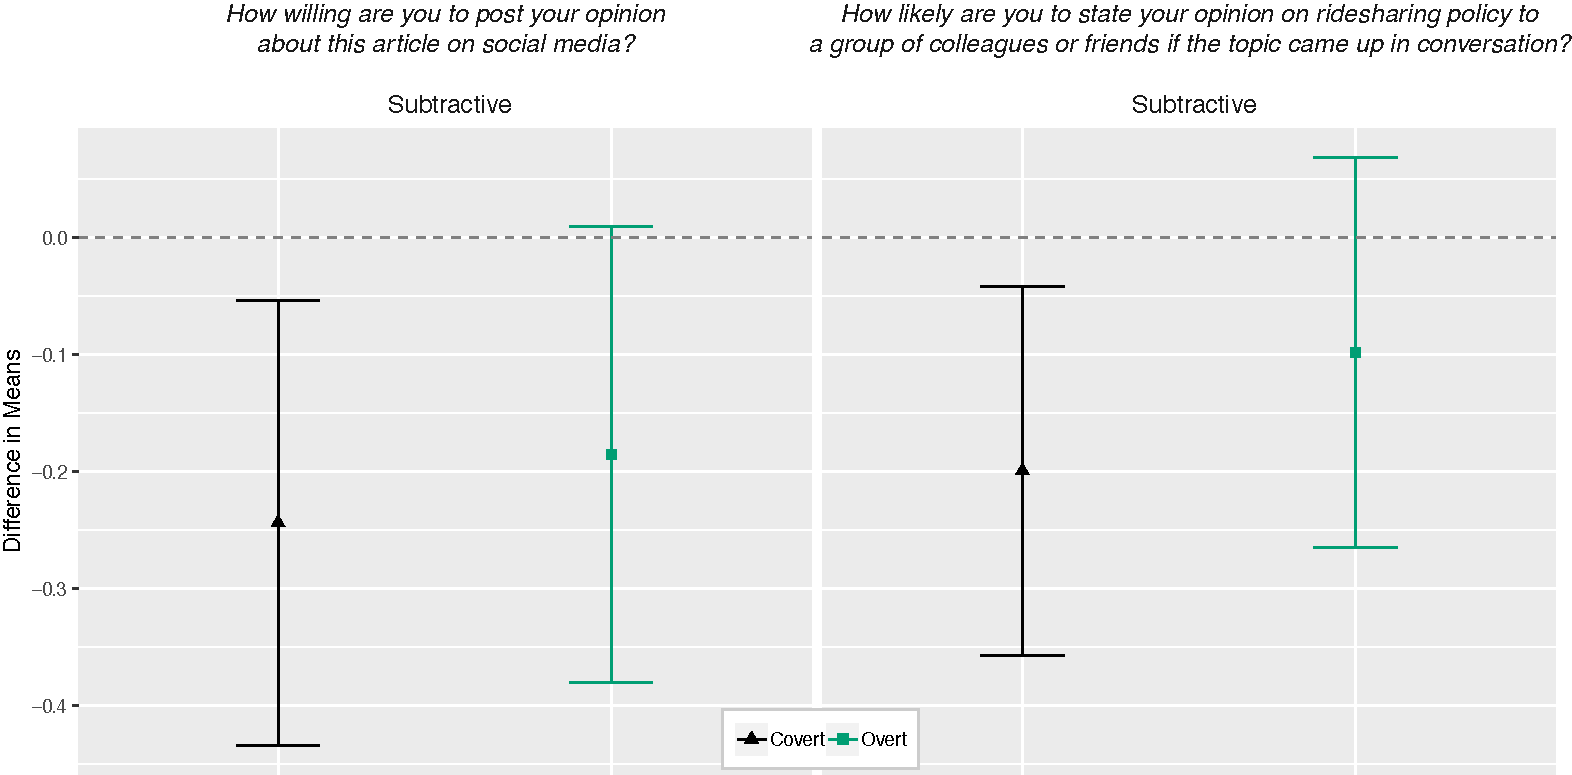
\includegraphics[width=.9\textwidth]{figures/ATE_opinion_expression.pdf}\\
        \label{ATE_opinion_expression}
    \end{center}
    \vspace{1em}
\end{minipage}

\begin{minipage}{\linewidth}
    \vspace{1em}
    \begin{center}
  \captionof{figure}{Nationalist Sentiment and Performance Legitimacy by Treatment Group}
        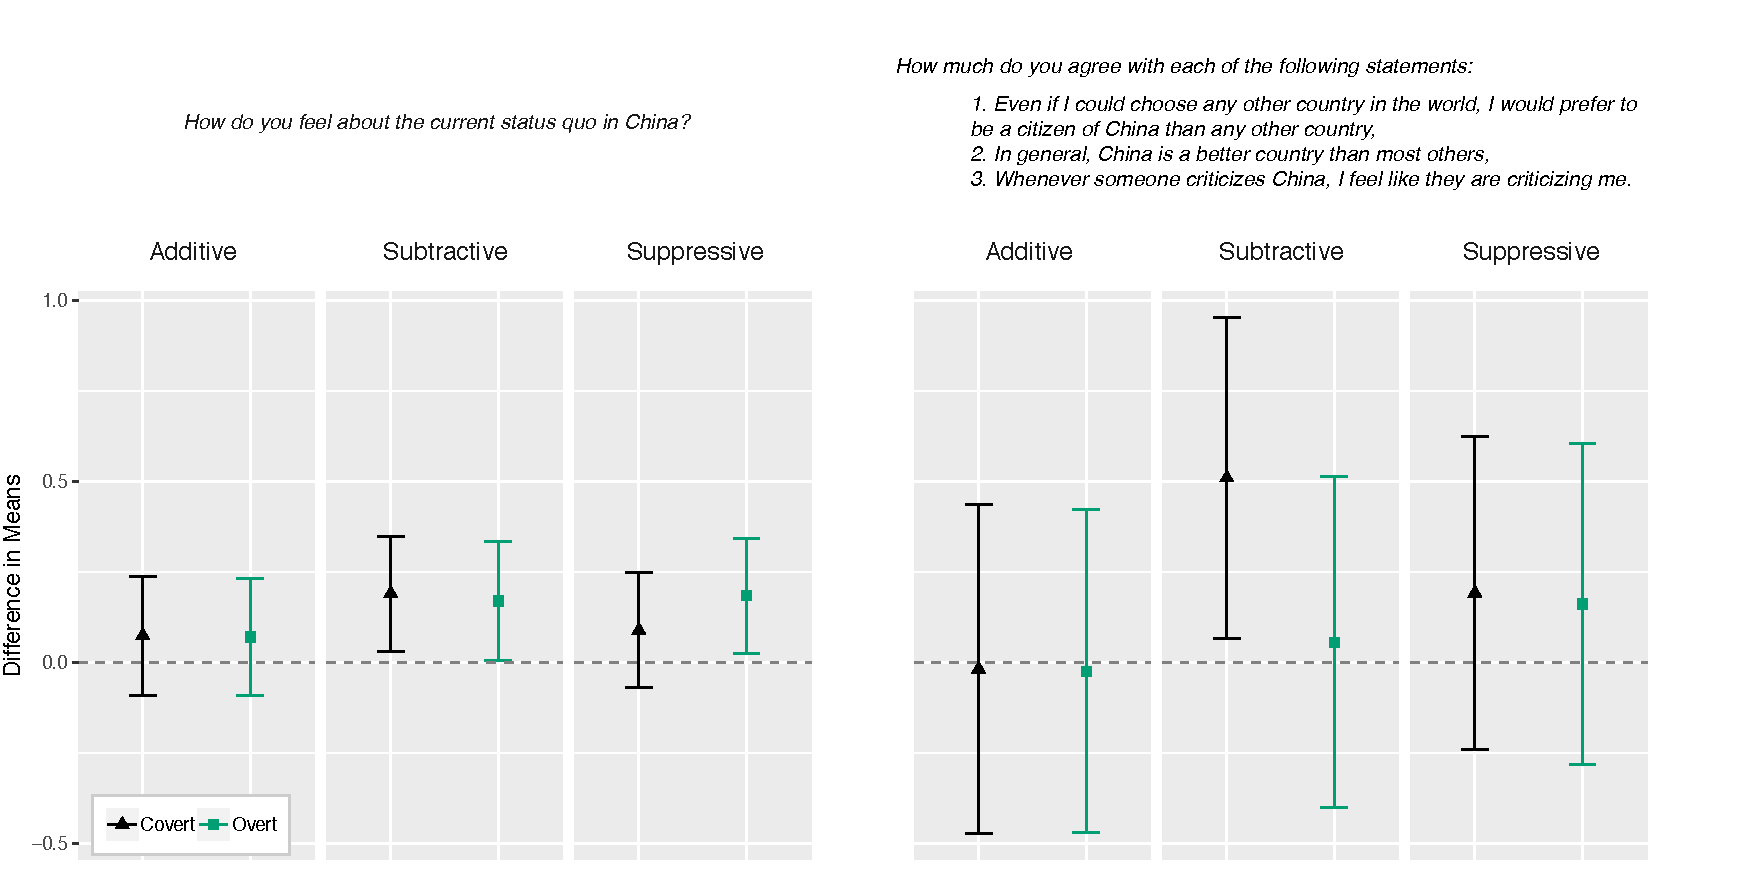
\includegraphics[width=\textwidth]{figures/ATE_legitimacy_nat_performance.pdf}\\
        \label{ATE_legitimacy_nat_performance}
    \end{center}
    \vspace{1em}
\end{minipage}

\begin{minipage}{\linewidth}
    \vspace{1em}
    \begin{center}
  		\captionof{figure}{Media Trust Measures for the Subtractive Treatment Group}
        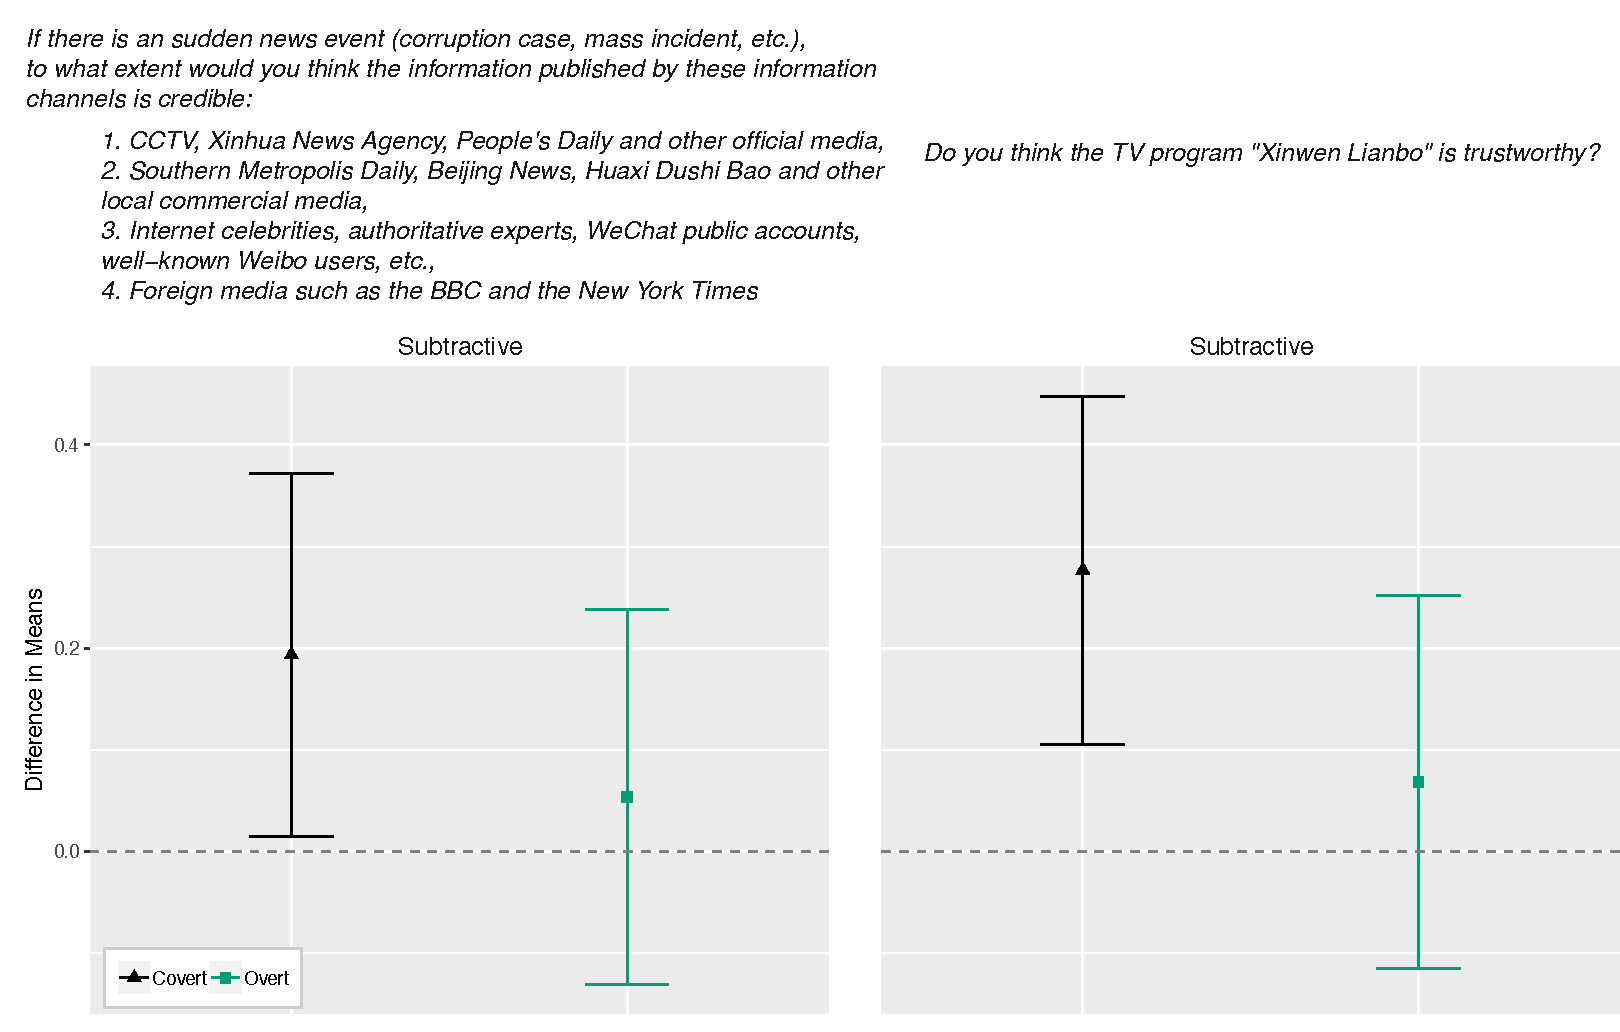
\includegraphics[width=.9\textwidth]{figures/ATE_media_trust.pdf}\\
        \label{ATE_media_trust}
    \end{center}
    \vspace{1em}
\end{minipage}

Opinions in the comment section were perceived as more credible in the three most effective treatment groups: covert subtractive, overt subtractive, and overt suppressive  (see \hyperref[ATE_credibility]{Figure \ref*{ATE_credibility}}). By more credible, I mean the comment sections were perceived as more representative of those held by society at large.

\begin{minipage}{\linewidth}
    \vspace{1em}
    \begin{center}
  		\captionof{figure}{Credibility by Treatment Group}
        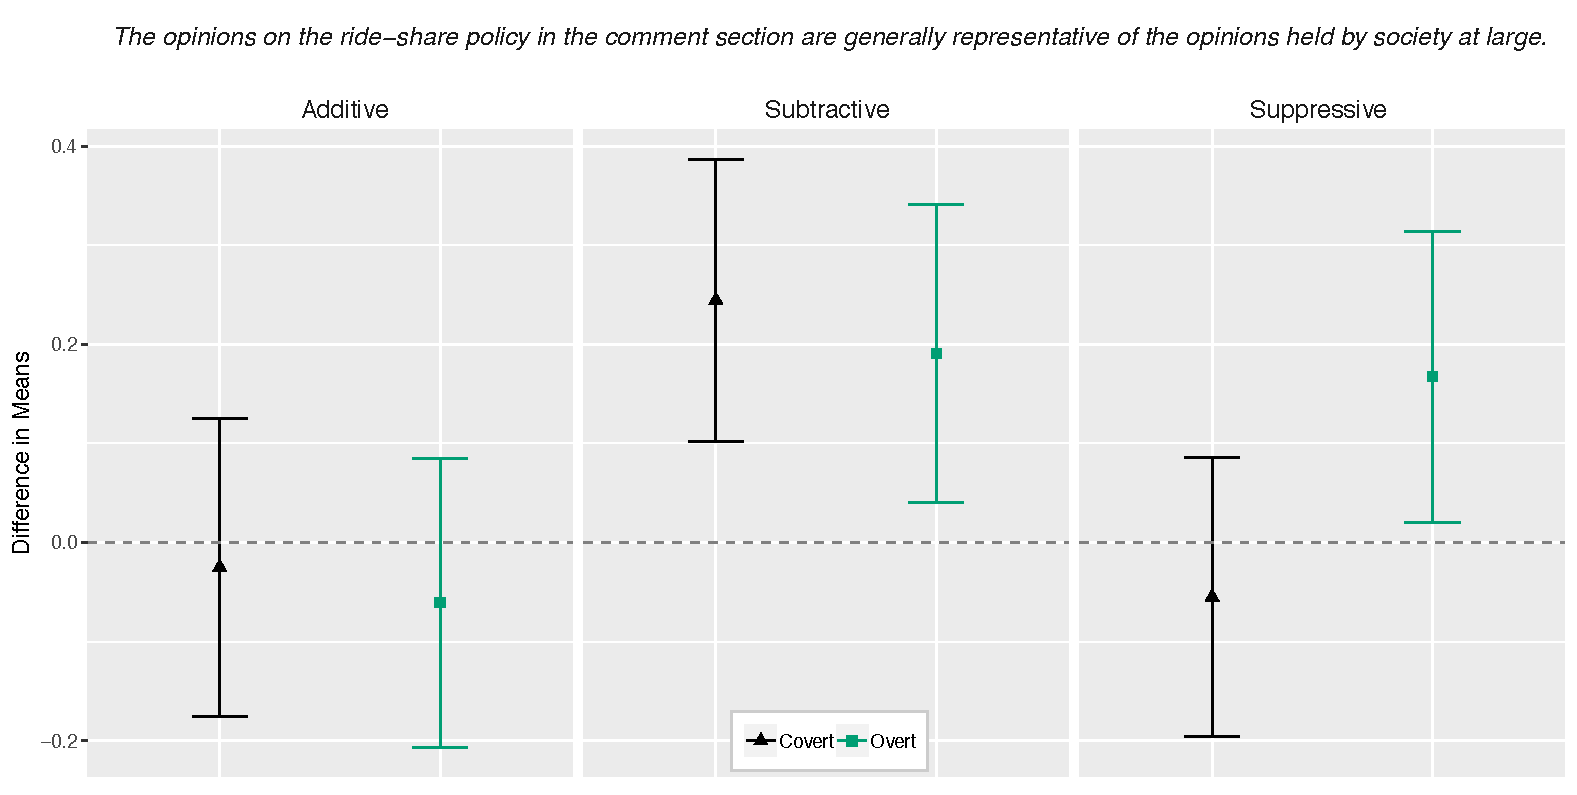
\includegraphics[width=.9\textwidth]{figures/ATE_credibility.pdf}\\
        \label{ATE_credibility}
    \end{center}
    \vspace{1em}
\end{minipage}

Evidence also suggests that suppressive information control is effective, but only in overt forms. This suggests that suppressive information control such as signaled surveillance is only effective when implied threats of repression are credible to individuals. In other words, users are afraid of possible retaliatory repression from the state but not private platform moderators.

Finally, I found evidence that overt additive information control can lead to poor user experience. According to two measures of user experience, I found that users expressed greater dissatisfaction with the platform when in the overt additive treatment.

While I sought out to test heterogenous effects, problems with data collection (likely due to the political sensitivity of the survey) left me with a smaller sample size than I originally intended. Because of this, there is not enough power to report results for heterogenous effects.

\begin{minipage}{\linewidth}
    \vspace{3em}
    \begin{center}
  		\captionof{figure}{User Experience Measures for the Additive Treatment Group}
        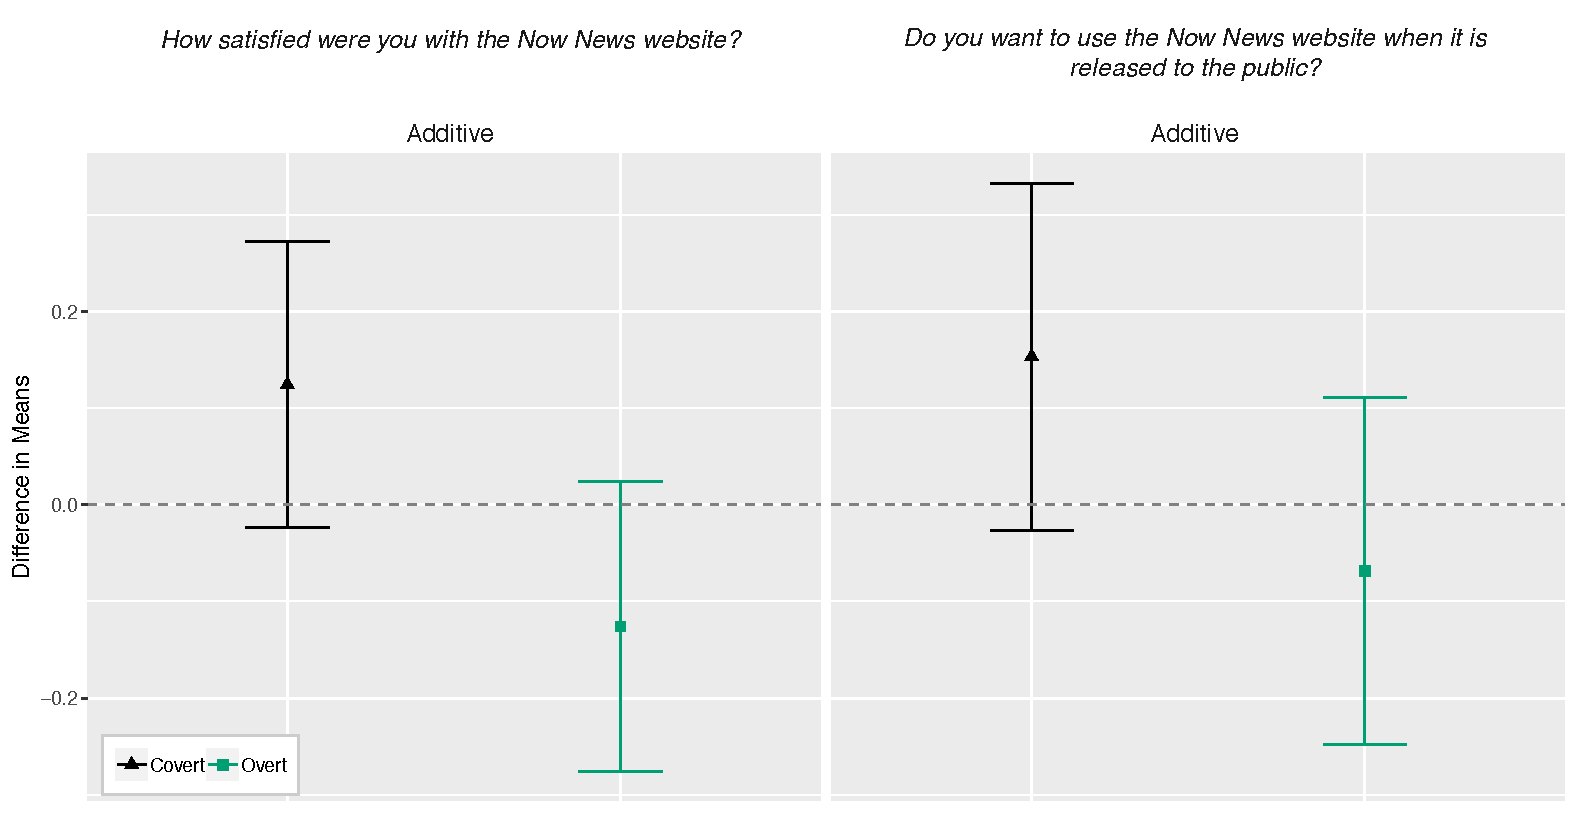
\includegraphics[width=.9\textwidth]{figures/ATE_ux.pdf}\\
        \label{ATE_ux}
    \end{center}
    \vspace{1em}
\end{minipage}


\newpage

\section{Appendix}\label{appendix}

\subsection{Article Text}\label{text}

\subsubsection{English}

Title: Timely Amend Internet-Based Ride-Share Policy\newline

\noindent Global Times Opinion: March 8, 2018 9:20 AM\newline

The internet-based ride-share policy has entered the full implementation stage. The policy is a major innovation and reform.

Internet-based ride-share services, as a classic model in the internet economy, is unique due to its cross-regional operations, which requires each locale to be innovative and flexible with their policies. However, the strictly local governance of the industry means that the cost of repeated auditing increases heavily and brings unnecessary burden to the services.

The internet-based ride-share policy is established to address these burdens and encourage the industry’s development. Therefore, local governments should reasonably relax their implementation policies in order to provide convenience transportation for passengers and counteract illegal taxi services by creating a sound resolution mechanism.

The internet-based ride-share policy aims to resolve safety problems and ensure the passengers’ legal rights by establishing a comprehensive mechanism that includes establishing barriers to entry on vehicle hardware, providing adequate insurance policies to drivers and ensuring rideshare services take more responsibility for vehicle safety.

Through a positive and cooperative mechanism which includes the government, the corporations, and the society, the remaining issues could be resolved.

\subsubsection{Mandarin}

\begin{minipage}{\linewidth}

\zh{适时给网约车政策打补丁}\newline

\noindent\zh{2018年03月08日 09:20 环球时报评论}\newline

\zh{网约车政策进入全面正式实施阶段,其制定是一场制度创新与改革。作为网络经济的一种典型模式,网约车有着跨地域经营的特点。因此,对属地管理制度要求灵活创新。但是,严格的属地管理特点意味着增加了各属地重复审核的行政成本,为网约车行业带来不必要的政策壁垒。}

\zh{网约车政策目的在于打破政策壁垒、鼓励行业发展。各地方的实施细应当适度松开政策口袋,在解决出行难的同时进一步改善经营管理,通过建立合理的疏导机制,统筹解决黑车这一社会顽疾。}

\zh{网约车政策也重点解决安全问题,通过建立一套完整的机制,包括对于车辆硬件建立准入门槛、设置合理的保险制度、明晰平台的责任等方式保障乘客合法权益。}

\zh{深化网约车行业管理体制改革,需要进一步拓宽思路,通过良性的制度设计以及政企合作、社会共治的模式来解决问题。}

\end{minipage}

\subsection{Comment Interface}
\vspace{-2em}
\begin{table}[H]
  \singlespacing
  \centering
  \caption{Ordinary Avatars}
  \begin{tabular}{|p{.125\textwidth}|p{.2\textwidth}|p{.45\textwidth}|p{.1\textwidth}|}
	\hline
	\textbf{Gender} & \textbf{Username} & \textbf{Username (English)} & \textbf{Avatar} \\ \hline
	Female & \zh{芽雅92} & Elegant Sprout 92 & \begin{minipage}{.2\textwidth}
\includegraphics[width=.45\linewidth, height=.45\linewidth]{figures/ordinary_avatars/f1.jpg}\end{minipage} \\ \hline
	Female & \zh{爱粽子的蚊子} & Dumpling-loving Mosquito & \begin{minipage}{.2\textwidth}
\includegraphics[width=.45\linewidth, height=.45\linewidth]{figures/ordinary_avatars/f2.jpg}\end{minipage} \\ \hline
	Female & \zh{老丸子89} & Old Meatball 89 & \begin{minipage}{.2\textwidth}
\includegraphics[width=.45\linewidth, height=.45\linewidth]{figures/ordinary_avatars/f3.jpg}\end{minipage} \\ \hline
	Female & \zh{雅思精解} & Elegant, thoughtful, energetic, liberated & \begin{minipage}{.2\textwidth}
\includegraphics[width=.45\linewidth, height=.45\linewidth]{figures/ordinary_avatars/f4.jpg}\end{minipage} \\ \hline
	Female & \zh{康尼岛大盗} & Coney Island Bandit & \begin{minipage}{.2\textwidth}
\includegraphics[width=.45\linewidth, height=.45\linewidth]{figures/ordinary_avatars/f5.jpg}\end{minipage} \\ \hline
	Female & \zh{等你的兔子} & Wait for your rabbit & \begin{minipage}{.2\textwidth}
\includegraphics[width=.45\linewidth, height=.45\linewidth]{figures/ordinary_avatars/f6.jpg}\end{minipage} \\ \hline
	Male & \zh{我心本尊} & Respect at the bottom of my heart & \begin{minipage}{.2\textwidth}
\includegraphics[width=.45\linewidth, height=.45\linewidth]{figures/ordinary_avatars/m1.jpg}\end{minipage} \\ \hline
	Male & \zh{章鱼丸子} & Octopus meatballs & \begin{minipage}{.2\textwidth}
\includegraphics[width=.45\linewidth, height=.45\linewidth]{figures/ordinary_avatars/m2.jpg}\end{minipage} \\ \hline
	Male & \zh{奇幻雨林} & Magical Rainforest & \begin{minipage}{.2\textwidth}
\includegraphics[width=.45\linewidth, height=.45\linewidth]{figures/ordinary_avatars/m3.jpg}\end{minipage} \\ \hline
	Male & \zh{那小子真帅44} & That guy is really handsome 44 & \begin{minipage}{.2\textwidth}
\includegraphics[width=.45\linewidth, height=.45\linewidth]{figures/ordinary_avatars/m4.jpg}\end{minipage} \\ \hline
	Male & \zh{太阳之光82} & Sunlight 82 & \begin{minipage}{.2\textwidth}
\includegraphics[width=.45\linewidth, height=.45\linewidth]{figures/ordinary_avatars/m5.jpg}\end{minipage} \\ \hline
	Male & \zh{萌面小怪兽} & Cute-faced Little Monster & \begin{minipage}{.2\textwidth}
\includegraphics[width=.45\linewidth, height=.45\linewidth]{figures/ordinary_avatars/m6.jpg}\end{minipage} \\ \hline
	Unspecified & \zh{爱玩的小胖} & Playful chubby thing & \begin{minipage}{.2\textwidth}
\includegraphics[width=.45\linewidth, height=.45\linewidth]{figures/ordinary_avatars/o1.jpg}\end{minipage} \\ \hline
	Unspecified & \zh{好人520} & Good person 520 (I love you) & \begin{minipage}{.2\textwidth}
\includegraphics[width=.45\linewidth, height=.45\linewidth]{figures/ordinary_avatars/o2.jpg}\end{minipage} \\ \hline
	Unspecified & \zh{可保平安} & Safe and sound & \begin{minipage}{.2\textwidth}
\includegraphics[width=.45\linewidth, height=.45\linewidth]{figures/ordinary_avatars/o3.jpg}\end{minipage} \\ \hline
  \end{tabular}
  \label{uids}
\end{table}

\begin{table}[H]
  \singlespacing
  \centering
  \caption{Government Avatars}
  \begin{tabular}{|p{.125\textwidth}|p{.2\textwidth}|p{.45\textwidth}|p{.1\textwidth}|}
	\hline
	\textbf{Gender} & \textbf{Username} & \textbf{Username (English)} & \textbf{Avatar} \\ \hline
	Unspecified & \zh{上海交警} & Shanghai Traffic Police & \begin{minipage}{.2\textwidth}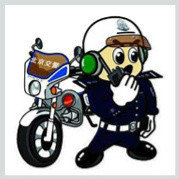
\includegraphics[width=.5\linewidth, height=.5\linewidth]{figures/govt_avatars/1.jpg}\end{minipage} \\ \hline
	Unspecified & \zh{上海交警网评员} & Shanghai Traffic Police commentator & \begin{minipage}{.2\textwidth}
\includegraphics[width=.5\linewidth, height=.5\linewidth]{figures/govt_avatars/2.jpg}\end{minipage} \\ \hline
	Unspecified & \zh{上海发布网评员} & Shanghai Publicity commentator & \begin{minipage}{.2\textwidth}
\includegraphics[width=.5\linewidth, height=.5\linewidth]{figures/govt_avatars/3.jpg}\end{minipage} \\ \hline
	Female & \zh{上海胡警官} & Shanghai Police Officer Hu & \begin{minipage}{.2\textwidth}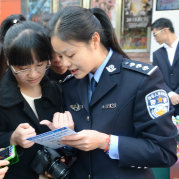
\includegraphics[width=.5\linewidth, height=.5\linewidth]{figures/govt_avatars/4.jpg}\end{minipage} \\ \hline
	Unspecified & \zh{中山民众镇青年志愿者} & Zhongshan Township Youth Volunteers & \begin{minipage}{.2\textwidth}
\includegraphics[width=.5\linewidth, height=.5\linewidth]{figures/govt_avatars/5.jpg}\end{minipage} \\ \hline
	Male & \zh{上海林警官} & Shanghai Police Officer Lin & \begin{minipage}{.2\textwidth}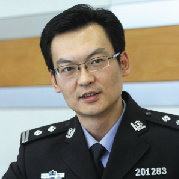
\includegraphics[width=.5\linewidth, height=.5\linewidth]{figures/govt_avatars/6.jpg}\end{minipage} \\ \hline
  \end{tabular}
  \label{uidgov}
\end{table}

\begin{table}[H]
    \singlespacing
    \centering
    \singlespacing
    \caption{All Comments}
    \label{comments}
    \resizebox{\textwidth}{!}{
    \begin{tabular}{|p{.14\textwidth}|p{.52\textwidth}|p{.28\textwidth}|p{.1\textwidth}|}
    \hline
        \textbf{Type} & \textbf{English} & \textbf{Chinese} & \textbf{Position} \\ \hline
        Critical & Isn't this kind of regulation is essentially prohibiting ride-share services? & \zh{这样管理还不如直接禁止网约车算了}  & 2 \\ \hline
        Critical & The number of illegal taxis in Shanghai never decreases. Damn. The authorities are all idling about. & \zh{上海的黑车什么时候少过 册那 管事的都是游手好闲。} & 12 \\ \hline
        Critical & Strict legislation, prevalent violation, selective enforcement, what's expected from the Communist Party.  & \zh{严格立法,普遍违法,选择执法,共党日常} & 13 \\ \hline
        Neutral & Ride-sharing cars need to display a sign, just like taxis do. It's easier for traffic police to supervise them this way. & \zh{网约车也要象的士一样,挂上标识,标注网约车三个字,方便交警管理。}  & 6 \\ \hline
        Neutral & The emergence of ride-sharing services reflects the development of the times. The emergence of a new industry certainly will come with lots of problems. The point is how to solve these problems.  & \zh{网约车是顺应时代发展的产物,一个新型行业的出现,必然会伴随很多问题,怎么处理好这些问题才是关键 } & 9 \\ \hline
        Neutral & I'd like to make a policy suggestion: passengers should be allowed to keep drivers' cell phones while they are in a taxi or using the Internet-based ride-share services like DIDI. Eight out of ten drivers are using their phones while driving. They don't even notice the traffic light when it turns green. & \zh{实名建议出台政策允许乘客打出租车或者滴滴这类的网约车时有权暂时替司机保管手机 十个司机里面八个边玩手机边开车 信号灯转绿了都不知道 } \hspace{.25em} 
\includegraphics[width=1.25em]{figures/emoji.png}& 15 \\ \hline
        Support & Support companies, support the economy, support reform, realize revitalization! & \zh{支持企业,发展经济,促进改革,实现振兴!}  & 1 \\ \hline
        Support & This policy will help the healthy development of the ride-sharing industry! & \zh{这个政策会推动网约车行业的健康发展!}  & 3 \\ \hline
        Support & Thank you Central Government for the good policy & \zh{感谢中央的好政策}  & 7 \\ \hline
        Astroturfing & The care for people from the Party and the nation is the warmest thing. & \zh{最给人温暖的,源自党和国家对人民的关怀。}  & 4 \\ \hline
        Astroturfing & The Party's policies are getting better and better, China's future will inevitably be bright. & \zh{党的政策越来越好,中国的未来必将更加美好 } & 5 \\ \hline
        Astroturfing & Listen to the Party and follow the Party! & \zh{听党话,跟党走!} & 8 \\ \hline
        Astroturfing & So many good policies make people full of hope for the future. & \zh{一项项利好政策的出台让人民对未来充满希望。} & 10 \\ \hline
        Astroturfing & Our country has introduced another policy that reflects a good deal of consultation [with the people]. & \zh{国家多出台一些像若干意见这些的政策。} & 11 \\ \hline
        Astroturfing & I hope that even more favorable policies are introduced to bring benefits to the people. & \zh{希望有更多优惠政策出台,让老百姓受益。} & 14 \\ \hline
    \end{tabular}
    }
\end{table}

\subsection{Survey Questionnaire}

\begin{table}[H]
    \singlespacing
    \centering
    \caption{Pre-Treatment Questions}
    \label{pre_treatment}
    \resizebox{\textwidth}{!}{
    \begin{tabular}{|c|p{.25\textwidth}|p{.45\textwidth}|p{.35\textwidth}|p{.18\textwidth}|}
    \hline
        \textbf{\#} & \textbf{Purpose} & \textbf{Question (EN)} & \textbf{Question (ZH)} & \textbf{Variable Type} \\\hline
        Q1 & Human Subjects Statement & - & - & - \\\hline
        Q2 & Browser Metadata & - & - & - \\\hline
        Q3 & Age & In what year were you born? & \zh{请问您是哪年出生的?} & Integer (1900-2001) \\\hline
        Q4 & Gender & What is your gender? & \zh{您的性别为:} & M, F, Other \\\hline
        Q5 & Province & In which province do you live? & \zh{您目前居住在哪个省?} & Multiple Choice \\\hline
        Q6 & Hukou & What type of hukou do you have? & \zh{您的户口为农业户口还是非农业户口?} & Urban/Rural \\\hline
        Q7 & Ethnicity & What ethnicity is on your identity card? & \zh{您属于哪个民族?(以身份证信息为准)} & Multiple Choice \\\hline
        Q8 & Years of education & How many years of education have you received? & \zh{您接受过多少年教育?} & Positive Integer \\\hline
        Q9 & Work Unit & In your career, what kind of work units have you been employed by? & \zh{您是否在以下这些类单位工作过?} & Multiple Choice \\\hline
        Q10 & Ideology & As a news media organization, we aim to provide our readers with the most trustworthy news sources. Generally speaking, what is your level of trust of these types of news sources? (central government official, entrepreneur, government official, doctor, banking executive, ordinary person, firefighter, university student) & \zh{作为一家新闻公司,我们希望为您提供最可靠的信息涞源。总体来说,您对以下这几种信息涞源的信任程度是怎样? (中央政府官员、企业家、地方政府官员、医生、银行高管、普通老百姓、消防员、大学生)} & - \\\hline
        Q11 & Newspaper Exposure & During a typical week, how many days do you read news in a printed newspaper? & \zh{在过去的一周内,您有多少天通过纸质媒体阅读新闻?} & Integer (1-7) \\\hline
        Q12 & Newspaper Exposure & Which of the following newspapers have you read in the last month? & \zh{在过去的一个月内,您曾阅读过下列哪些报纸?} & Multiple Answer \\\hline
        Q13 & Television Exposure & During a typical week, how many days do you watch news on TV? & \zh{在过去的一周内,您有多少天通过电视观看新闻?} & Integer (1-7) \\\hline
        Q14 & Television Exposure & Which of the following television news programs have you watched in the last month? & \zh{在过去的一个月内,您曾观看过下列哪些新闻节目?} & Multiple Answer \\\hline
        Q15 & Internet News Exposure & During a typical week, how many days do you watch or read news on the Internet? & \zh{在过去的一周内,您有多少天通过互联网获取新闻?} & Integer (1-7) \\\hline
        Q16 & Internet News Exposure & Which of the following news websites have you visited in the last month? & \zh{在过去的一个月内,您曾访问过下列哪些新闻网站?} & Multiple Answer \\\hline
        Q17 & Social Media Exposure & During a typical week, how many days do you watch or read news on social media (i.e. Weibo, WeChat, QQ, etc.)? & \zh{在过去的一周内,您有多少天通过社交媒体(比如微信、微博、QQ、等)获取新闻?} & Integer (1-7) \\\hline
        Q18 & Social Media Exposure & Which of the following social networking platforms have you visited in the last month? & \zh{在过去的一个月内,您曾访问过下列哪些社交媒体平台?} & Multiple Answer \\\hline
        Q19 & Ideology (Xi Jinping App) & Which of the following apps have you downloaded? & \zh{您下载过以下哪些移动应用程序(APP)?} & Multiple Answer \\\hline
        Q20 & Block Explainer & The next few questions will test your understanding of past and present hot news events. The following questions range from very easy to very difficult. Please answer to the best of your ability and don't worry about getting every question right. & \zh{接下来的几个问题将测试您对过去和近期热点事件的了解程度。以下问题难度各异,请按照您所知道的情况回答,回答时不必担心正确率。} &  \\\hline
        Q21 & Political Knowledge & Where was the 2016 G20 Conference was held? & \zh{以下哪座城市是2016年G20峰会的举办地?} & Multiple Choice \\\hline
        Q22 & Political Knowledge & In what year did Hong Kong return to the motherland? & \zh{香港在哪一年回归祖国?} & Multiple Choice \\\hline
        Q23 & Political Knowledge & Which of the following political slogans were not created under President Xi Jinping's leadership? & \zh{以下哪个理念不是在习近平的领导下提出的?} & Multiple Choice \\\hline
        Q24 & Political Knowledge & Who was China's Premier from 2003-2013? (Wang Qishan, Li Keqiang, Xi Jinping, Hu Jintao, Wen Jiabao, Jiang Zemin) & \zh{下列哪位国家领导人曾在2003至2013年间担任中华人民共和国总理?} & Multiple Choice \\\hline
        Q25 & Political Knowledge & In 2017 China had a border conflict with which country? & \zh{中国曾在2017年与下列哪个国家发生过边界冲突?} & Multiple Choice \\\hline
        Q26 & Political Knowledge & Do you know the name of your provincial-level party secretary's name? & \zh{您是否知道您所住地区省(市、自治区)党委书记的名字?} & Yes, No \\\hline
        \end{tabular}
    }
\end{table}

\begin{table}[H]
    \singlespacing
    \centering
    \caption{Post-Treatment Questions}
    \label{post_treatment_1}
    \resizebox{\textwidth}{!}{
    \begin{tabular}{|c|p{.15\textwidth}|p{.48\textwidth}|p{.38\textwidth}|l|}
    \hline
        \textbf{\#} & \textbf{Purpose} & \textbf{Question (EN)} & \textbf{Question (ZH)} & \textbf{Variable Type} \\\hline
        Q29 & Distractor & How often do you make purchases on Taobao? & \zh{您在淘宝上购物的频率:} & Multiple Choice \\\hline
        Q30 & Agreement with Policy & We are very interested in your opinion. Could you please share with us your opinion about the new ride share policy? Please write two or more sentences. & \zh{我们对您的观点很感兴趣,请您与我们分享您有关网约车政策的观点。请您提供两句话以上的评价。} & Open-ended \\\hline
        Q31 & Agreement with Policy & Recall the article you just read. If you had to guess, what position would most of your peers take on the ride-share policy discussed in the article? (very strongly support, strongly support, support, oppose, strongly oppose, very strongly oppose) & \zh{结合您刚刚阅读的文章,请您做出以下猜测,您周围的人对文章中提到的网约车政策持有怎样的立场?} & Multiple Choice \\\hline
        Q32 & Agreement with Policy & Recall the article you just read. What is your position on the ride-share policy discussed in the article? (very strongly support, strongly support, support, neutral, oppose, strongly oppose, very strongly oppose) & \zh{结合您刚刚阅读的文章,您对文章中提到的网约车政策持有怎样的立场?} & Multiple Choice \\\hline
        Q33 & Self-expression & How willing are you to post your opinion about this article on social media? (very unwilling, unwilling, slightly unwilling, neutral, slightly willing, willing, very willing) & \zh{您是否愿意将您对此文章的观点发布在社交媒体上?} & Multiple Choice \\\hline
        Q34 & Self-expression & How likely are you to state your opinion on ridesharing policy to a group of colleagues or friends if the topic came up in conversation? (very likely, likely, somewhat likely, neutral, somewhat unlikely, likely, very likely) & \zh{如果有人在谈话中提起此话题,你有多大可能向同事或朋友陈述你对网约车政策的意见?} & Multiple Choice \\\hline
        Q35 & Credibility & The opinions on the ride-share policy in the comment section are generally representative of the opinions held by society at large. & \zh{评论区的各种意见总体代表了社会对网约车的意见。} & Multiple Choice \\\hline
        Q36 & Discourse Competition & How much do you agree with each of the following points? 1) There are many different opinions in the comment area. 2) People with different opinions are willing to actively participate in the discussion. 3) Some opinions in the comment section are overrepresented. 4) The discussion in the comment area is biased towards one point of view. & \zh{请问您在多大程度上同意下面的观点:1)评论区有许多不同的观点。2)持有不同观点的人愿意积极参与讨论。3)某些意见在评论区中过多。4)评论区的讨论偏向于一个观点。} & Multiple Choice \\\hline
        Q37 & Discourse Competition/Credibility & Please share a bit about your experience with the article's comment area. Please write two or more sentences. & \zh{请您分享一下您对文章评论区域的阅读与使用体验。请您提供两句话以上的评价。} & Open-ended \\\hline
        Q38 & Block Explainer & Some readers prefer to read articles from Party media outlets while others prefer more independent media outlets. This section will help us understand how to best serve each type of reader. & \zh{有些读者喜欢阅读官媒的新闻,而有些读者更喜欢阅读商业媒体的新闻。 接下来这部分调查是关于您的阅读偏好。} & - \\\hline
        Q39 & Trust in State Media & Do you think the TV program ``Xinwen Lianbo'' is trustworthy? (very trustworthy, trustworthy, somewhat trustworthy, neutral, somewhat untrustworthy, untrustworthy, very untrustworthy) & \zh{您认为《新闻联播》节目内容可信度如何?} & Multiple Choice \\\hline
        Q40 & Trust in State Media & If there is an sudden news event (corruption case, mass incident, etc.), to what extent would you think the information published by these information channels is credible: 1) CCTV, Xinhua News Agency, People's Daily and other official media, 2) Southern Metropolis Daily, Beijing News, Huaxi Dushi Bao and other local commercial media, 3) Internet celebrities, authoritative experts, WeChat public accounts, well-known Weibo users, etc., 4) Foreign media such as the BBC and the New York Times & \zh{假如发生突发事件(腐败案件、群体性事件等),下面这些信息渠道发布的信息您在多大程度上觉得可信?1) 央视、新华社、人民日报等官方媒体, 2) 南方都市报、新京报、华西都市报等地方性商业媒体, 3) 网络名人、权威专家的微信公众号、知名微博等自媒体, 4) BBC、纽约时报等国外媒体} & Multiple Choice \\\hline
    \end{tabular}
    }
\end{table}

\begin{table}[H]
    \singlespacing
    \caption{Post-Treatment Questions (continued)}
    \label{post_treatment_2}
    \resizebox{\textwidth}{!}{
    \begin{tabular}{|c|p{.18\textwidth}|p{.52\textwidth}|p{.4\textwidth}|p{.12\textwidth}|}
    \hline
        \textbf{\#} & \textbf{Purpose} & \textbf{Question (EN)} & \textbf{Question (ZH)} & \textbf{Variable Type} \\\hline
        Q41 & Trust in State Media & Could you please explain your answers to the previous two questions? & \zh{您能解释一下您对前两个问题的答案吗?请您提供两句话以上的评价。} & Open-ended \\\hline
        Q42 & Legitimacy & Do you agree with the following: ``Our government is working for the people and serving their needs'' (strongly agree, agree, somewhat agree, neutral, somewhat disagree, disagree, very much disagree) & \zh{您同意下列说法吗?``总的来说,我们的政府在响应人民的要求,为人民做事。}'' & Multiple Choice \\\hline
        Q43 & Legitimacy & How do you feel about the current status quo in China? (very satisfied, satisfied, somewhat satisfied, neutral, somewhat dissatisfied, dissatisfied, very dissatisfied) & \zh{您对中国目前总体现状感觉如何?}  & Multiple Choice \\\hline
        Q44 & Legitimacy & Could you please explain your answers to the previous two questions? Please write two or more sentences. & \zh{您能解释一下您对前两个问题的答案吗?请您提供两句话以上的评价。} & Open-ended \\\hline
        Q45 & Block Explainer & In order to improve our products as much as possible, we invite you to answer the following questions about your user experience. Any suggestions you have will be incredibly helpful to us, thank you for your sincere feedback. & \zh{为了尽可能优化我们的产品, 我们诚邀您对以下使用体验问题进行回答。您的任何反馈都将会为我们提供巨大的帮助,感谢您的真诚反馈。} & - \\\hline
        Q46 & User Satisfaction & How satisfied were you with the Now News website? (Very satisfied, satisfied, somewhat satisfied, neutral, somewhat unsatisfied, unsatisfied, very unsatisfied) & \zh{您对Now新闻网的满意程度:} & Multiple Choice \\\hline
        Q47 & User Satisfaction & Do you want to use the Now News website when it is released to the public? (Really want to use, want to use, somewhat want to use, indifferent, somewhat don't want to use, don't want to use, really do not want to use) & \zh{在Now新闻正式发布时,您是否想使用这个网站?} & Multiple Choice \\\hline
        Q48 & User Satisfaction & Could you explain in a few sentences your answers to the previous two questions? &\zh{您能解释一下您对前两个问题的答案吗?请您提供两句话以上的评价。} & Open-ended \\\hline
        Q49 & Block Explainer & Readers have many different perspectives on international politics. This section will help us understand how to provide a wide range of perspectives to each type of reader. & \zh{在我们的新闻报道中包含了许多有关国际关系的观点。作为一个对读者来说十分重要的话题,我们将在下一部分的调查中就中国的国际关系向您提出一些问题。} & - \\\hline
        Q50 & Nationalism & How much do you agree with each of the following statements: 1) Even if I could choose any other country in the world, I would prefer to be a citizen of China than any other country, 2) In general, China is a better country than most others, 3) Whenever someone criticizes China, I feel like they are criticizing me. & \zh{请问您在多大程度上同意下面的观点:1)即使可以选择世界上任何国家,我也更愿意做中国公民。2)总的来说,中国比其他大部分国家都好。3)别人批评中国时,就像在批评我自己} & Multiple Choice \\\hline
        Q51 & Nationalism & Could you please explain your answers to the previous question? Please write two or more sentences. & \zh{您能解释一下您对上一个问题的答案吗?请您提供三句话以上的评价。}  & Open-ended \\\hline
        Q52 & Distractor & Which of the following mobile operating systems do you use? & \zh{您使用以下哪种手机操作系统?} & Multiple Choice \\\hline
        Q53 & Collective Action & How likely are you to sign a petition to support something you highly in favor of? (very likely, likely, somewhat likely, neutral, somewhat unlikely, likely, very likely) & \zh{您有多大可能会通过联名上书来表达您的观点和信念?} & Multiple Choice \\\hline
        Q54 & Collective Action & How likely are you to join a petition to support something you are highly in favor of? (very likely, likely, somewhat likely, neutral, somewhat unlikely, likely, very likely) & \zh{您有多大可能会通过参加信访、上访来表达您的观点和信念?} & Multiple Choice \\\hline
        Q55 & Collective Action & How likely are you to join a march to support something you are highly in favor of? (very likely, likely, somewhat likely, neutral, somewhat unlikely, likely, very likely) & \zh{您有多大可能会通过参加游行集会来表达您的观点和信念?} & Multiple Choice \\\hline
        Q56 & Collective Action & Could you explain in a few sentences your answers to the previous three questions? & \zh{您能解释一下您对前三个问题的答案吗?请您提供三句话以上的评价。 }& Open-ended \\\hline
    \end{tabular}
    }
\end{table}

\begin{table}[H]
    \singlespacing
    \centering
    \caption{Manipulation and Attention Checks}
    \label{manip_check}
    \resizebox{\textwidth}{!}{
    \begin{tabular}{|c|p{.15\textwidth}|p{.45\textwidth}|p{.35\textwidth}|l|}
    \hline
        \textbf{\#} & \textbf{Purpose} & \textbf{Question (EN)} & \textbf{Question (ZH)} & \textbf{Variable Type} \\\hline
        Q57 & Manipulation & Which notice below was displayed in the comment area? & \zh{评论区中出现过哪个通知?} & Multiple Choice \\\hline
        Q58 & Manipulation Check & Were there any comments on the official account of the party and government agencies (such as the public security bureau, the Communist Youth League, etc.) in the comment area (with the V logo)? & \zh{在评论区中有没有经过认证的党政机关(例如公安、共青团、等)官方账号(带有V标志)的评论?} & Multiple Choice \\\hline
        Q59 & Attention & What is the topic of this article? & \zh{这篇报道的主题是什么?} & Multiple Choice \\\hline
        Q60 & Attention & The price of the ride-sharing services and taxis may be different. We want to know your point of view. To prove that you are paying attention, please choose the third answer: & \zh{网约车和出租车的价格可能不同,我们想知道您的观点。为了证明您正在关注,请选择第三个答案:} & Multiple Choice \\\hline
        Q61 & Attention & Was this image displayed in the article? & \zh{文章中是否出现过该图片?} & Multiple Choice \\\hline
        Q62 & Manipulation & If you had to guess, how many comments in the comment section of the article were in favor of the ride-share policy? & \zh{请您做出猜测,文章的评论区有多少赞成网约车政策的评论?} & Multiple Choice \\\hline
    \end{tabular}
    }
\end{table}


\begin{table}[H]
  \singlespacing
  \centering
  \caption{Media Exposure Sources}
  \resizebox{\textwidth}{!}{
  \begin{tabular}{|c|c|c|c|}
	\hline
		\textbf{Name (ZH)} & \textbf{Name (EN)} & \textbf{Source Type} & \textbf{Medium} \\ \hline
        \zh{参考消息} & Reference News & Semiofficial & Newspaper \\ \hline
        \zh{经济日报} & Economic Daily & Semiofficial & Newspaper \\ \hline
        \zh{华商报} & Chinese Business Paper & Semiofficial & Newspaper \\ \hline
        \zh{人民日报} & People's Daily & Official & Newspaper \\ \hline
        \zh{工人日报} & Workers' Daily & Official & Newspaper \\ \hline
        \zh{环球时报} & Global Times & Official & Newspaper \\ \hline
        \zh{经济观察报} & Economic Observer & Commercialized & Newspaper \\ \hline
        \zh{21世纪经济报道} & 21st Century Economic Report & Commercialized & Newspaper \\ \hline
        \zh{财经时报} & Business Times & Commercialized & Newspaper \\ \hline
        \zh{人民网} & People's Network & Official & Website \\ \hline
        \zh{央视网} & CCTV & Official & Website \\ \hline
        \zh{新华网} & xinhuanet & Official & Website \\ \hline
        \zh{网易新闻} & NetEase & Commercialized & Website \\ \hline
        \zh{新浪新闻} & Sina News & Commercialized & Website \\ \hline
        \zh{今日头条} & Toutiao & Commercialized & Website \\ \hline
        \zh{腾讯新闻} & Tencent News & Commercialized & Website \\ \hline
        \zh{搜狐新闻} & Sohu News & Commercialized & Website \\ \hline
        \zh{凤凰网} & Phoenix News & Commercialized & Website \\ \hline
        \zh{纽约时报} & The New York Times & Blocked & Website \\ \hline
        \zh{明报新闻网} & Mingpao & Blocked & Website \\ \hline
        \zh{苹果日报} & Apple Daily & Blocked & Website \\ \hline
        \zh{微信} & WeChat & Domestic & Social Media Platform \\ \hline
        \zh{新浪微博} & Sina Weibo & Domestic & Social Media Platform \\ \hline
        \zh{腾讯QQ} & Tencent QQ & Domestic & Social Media Platform \\ \hline
        \zh{百度贴吧} & Baidu Tieba & Domestic & Social Media Platform \\ \hline
        \zh{豆瓣} & Douban & Domestic & Social Media Platform \\ \hline
        \zh{知乎} & Zhihu & Domestic & Social Media Platform \\ \hline
        \zh{Facebook (脸书)} & Facebook & Blocked & Social Media Platform \\ \hline
        \zh{Twitter (推特)} & Twitter & Blocked & Social Media Platform \\ \hline
        \zh{Instagram} & Instagram & Blocked & Social Media Platform \\ \hline
        \zh{新闻联播} & Xīnwén Liánbò & - & Television Program \\ \hline
        \zh{焦点访谈} & Jiāodiǎn Gǎngtán & - & Television Program \\ \hline
        \zh{今日关注} & Jīnrì Guānzhù & - & Television Program \\ \hline
        \zh{海峡两岸} & Hǎixiá Liǎng'àn & - & Television Program \\ \hline
        \zh{新闻30分} & Xīnwén 30 Fēn & - & Television Program \\ \hline
        \zh{中国新闻} & Zhōngguó Xīnwén & - & Television Program \\ \hline
        \zh{今日亚洲} & Jīnrì Yàzhōu & - & Television Program \\ \hline
        \zh{中国舆论场} & Zhōngguó Yúlùn Chǎng & - & Television Program \\ \hline
        \zh{深度国际} & Shēndù Guójì & - & Television Program \\ \hline
  \end{tabular}
  }
  \label{exposure}
\end{table}

\newpage

\subsection{Coding Diagrams for Comments and Open-Ended Responses}\label{diags}

\begin{figure}[H]
  \centering
  \caption{Collective Action Coding Diagram}
  \vspace{1em}
  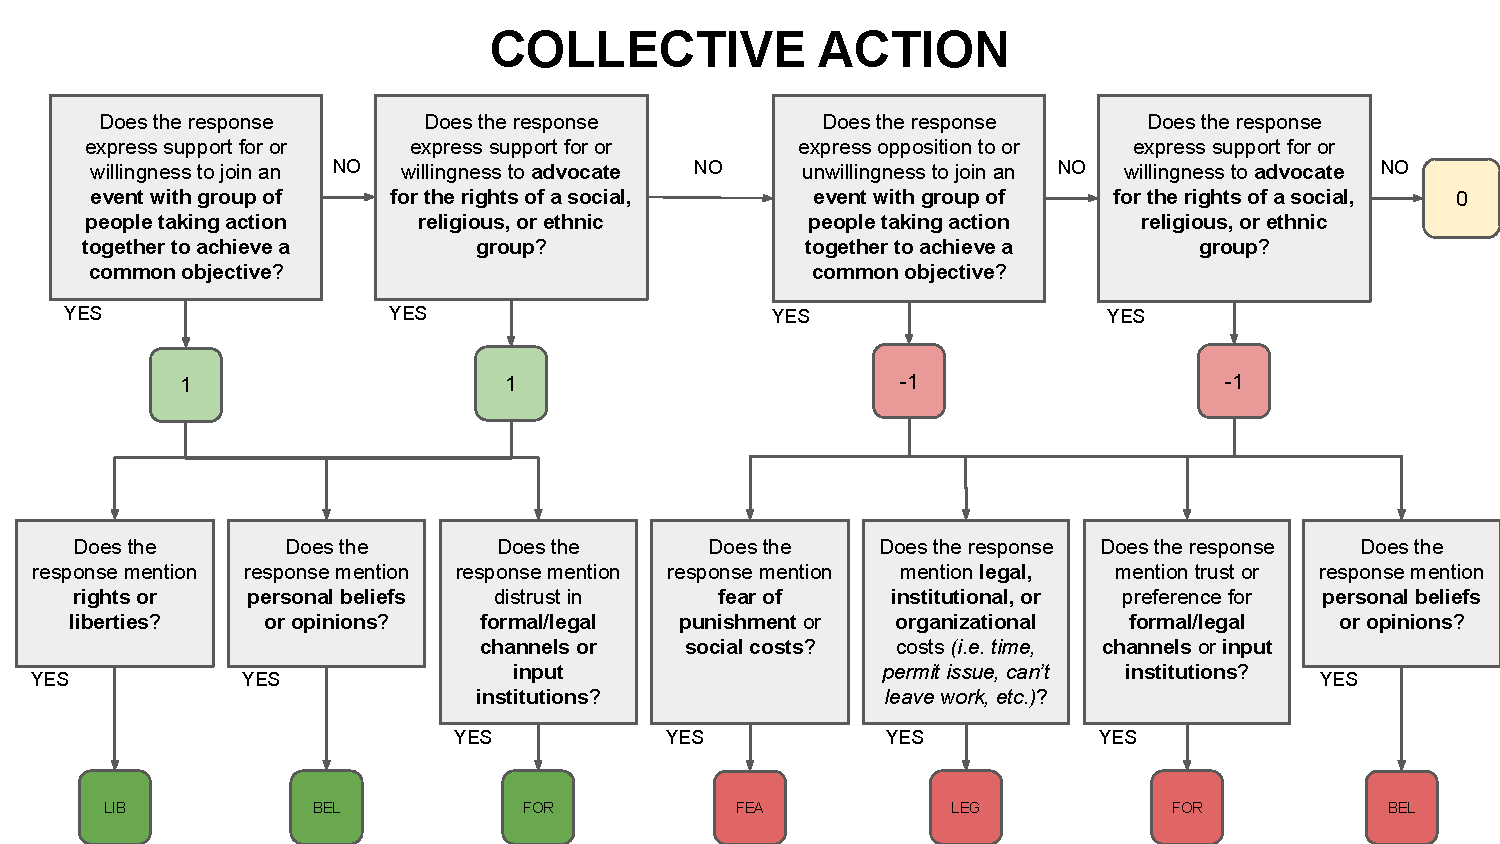
\includegraphics[width=\textwidth]{figures/coding_diagrams/collective_action.pdf}
  \label{collective_action}
\end{figure}

\begin{figure}[H]
  \centering
  \caption{Legitimacy Coding Diagram}
  \vspace{1em}
  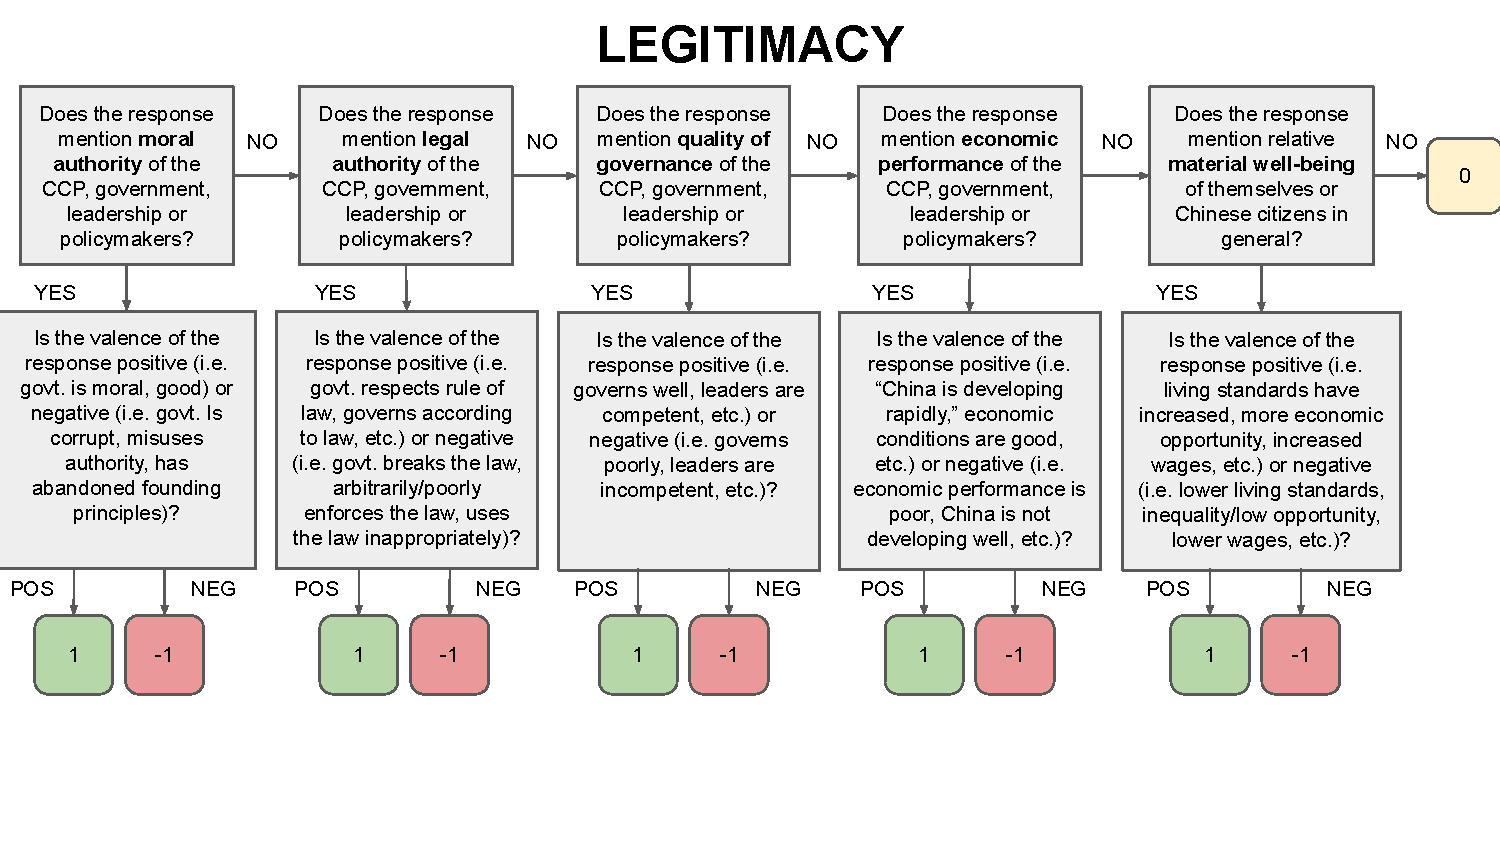
\includegraphics[width=\textwidth]{figures/coding_diagrams/legitimacy.pdf}
  \label{legitimacy}
\end{figure}

\begin{figure}[H]
  \centering
  \caption{User Satisfaction and State Media Affinity Coding Diagrams}
  \vspace{1em}
  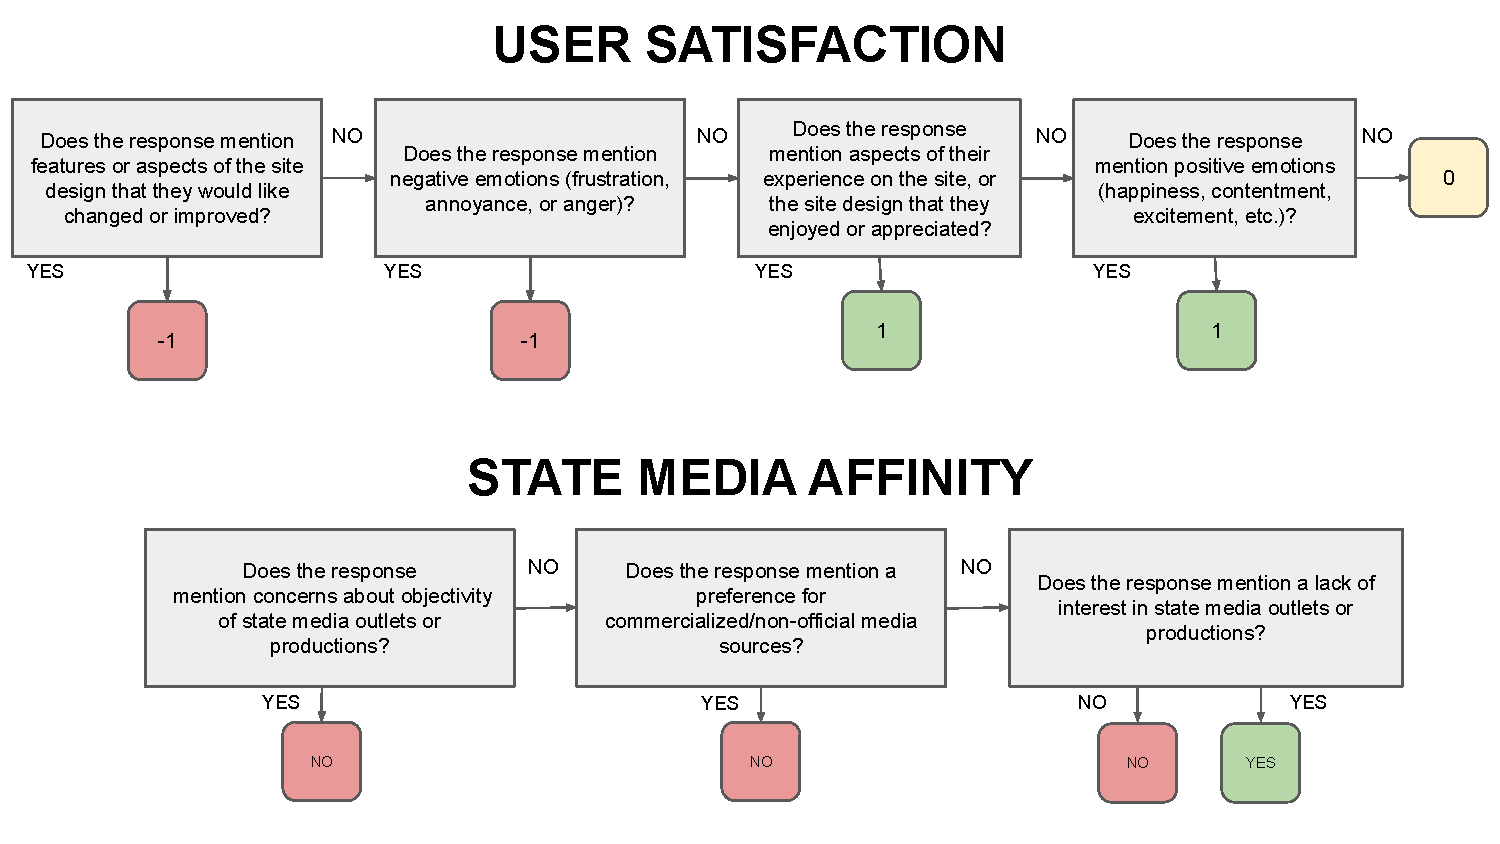
\includegraphics[width=\textwidth]{figures/coding_diagrams/user_sat_state_media.pdf}
  \label{user_sat_state_media}
\end{figure}

\begin{figure}[H]
  \centering
  \caption{Favorability Coding Diagram}
  \vspace{1em}
  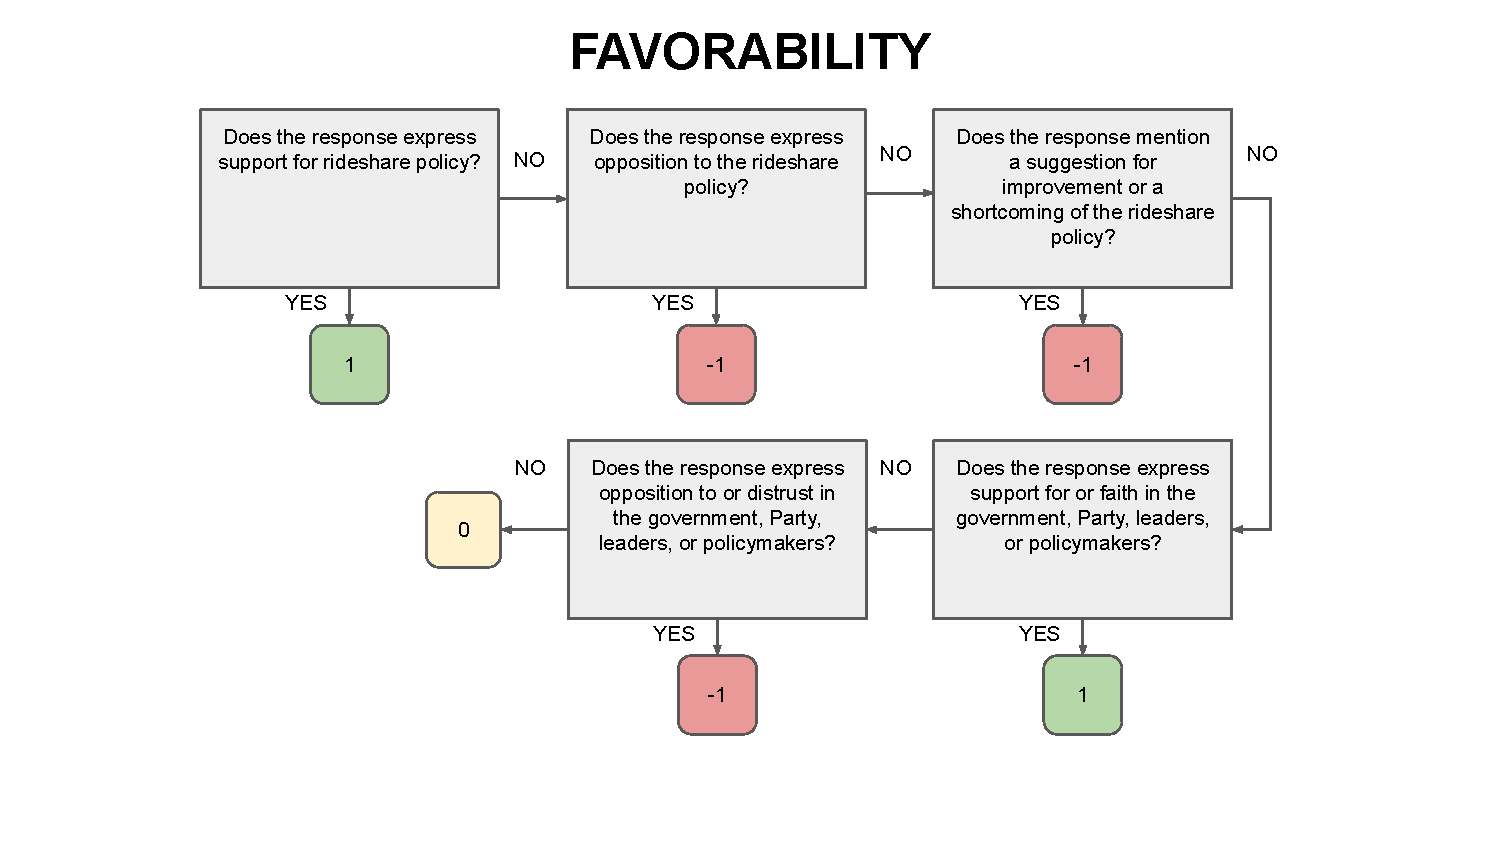
\includegraphics[width=\textwidth]{figures/coding_diagrams/favorability.pdf}
  \label{favorability}
\end{figure}

\begin{figure}[H]
  \centering
  \caption{Nationalism Coding Diagram}
  \vspace{1em}
  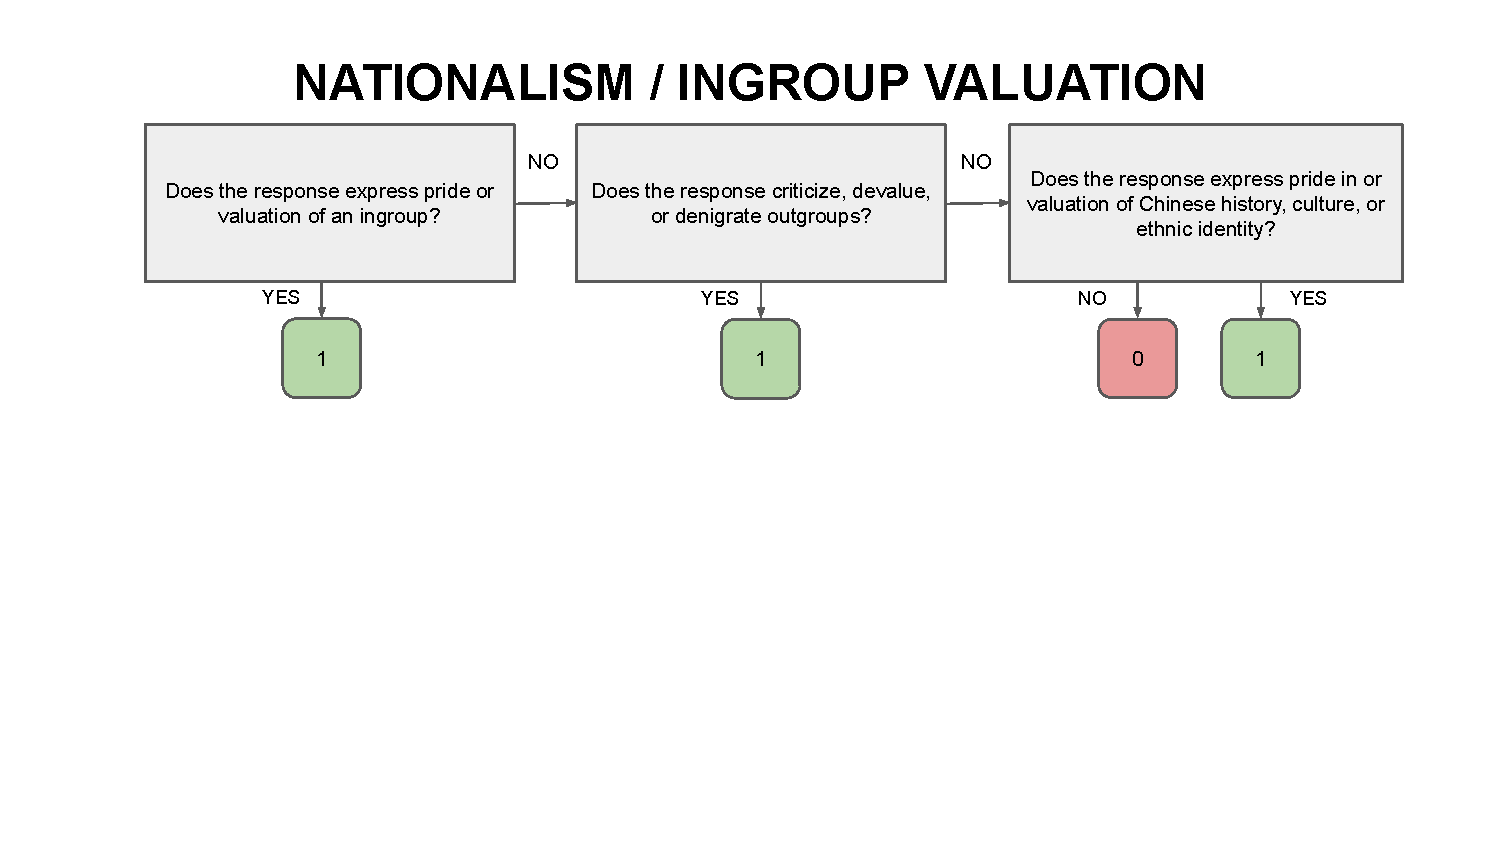
\includegraphics[width=\textwidth]{figures/coding_diagrams/nationalism.pdf}
  \label{nationalism}
\end{figure}

\begin{figure}[H]
  \centering
  \caption{Discourse Competition Coding Diagram}
  \vspace{1em}
  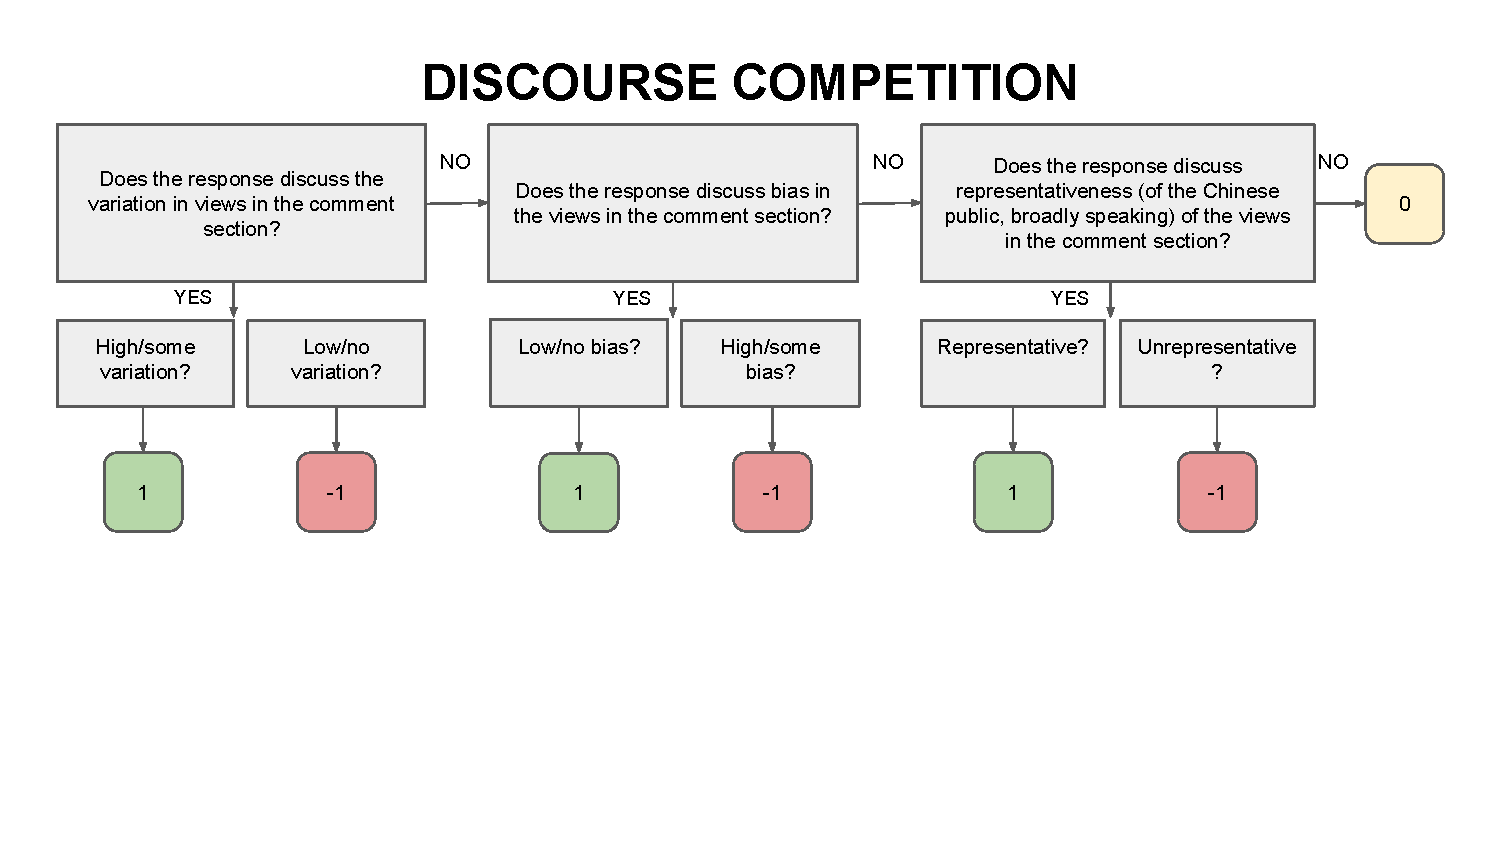
\includegraphics[width=\textwidth]{figures/coding_diagrams/discourse_competition.pdf}
  \label{discourse_competition}
\end{figure}

\newpage

\bibliographystyle{apacite}
\bibliography{info_control}

\end{document}